% =====================================================================
%  A Conditional Reduction of the 4D Pure Yang–Mills Mass Gap
%  Build:  xelatex/pdflatex main.tex  (run twice)
% =====================================================================
\documentclass[11pt,a4paper]{article}

\usepackage[T1]{fontenc}
\usepackage[utf8]{inputenc}
\usepackage{lmodern}
\usepackage[margin=2.5cm,top=2.2cm,bottom=2.4cm,headsep=14pt]{geometry}
\usepackage{amsmath,amssymb,amsthm,mathtools,bm}
\usepackage{microtype}
\usepackage[table]{xcolor}
\usepackage{booktabs,array,tabularx,longtable}
\usepackage{graphicx}
\usepackage{tikz}
\usetikzlibrary{arrows.meta,positioning,calc,shapes.geometric,decorations.pathreplacing,patterns}
\usepackage{tcolorbox}
\tcbuselibrary{skins,breakable}
\usepackage{enumitem}
\usepackage{multicol}
\usepackage{CJKutf8}
\usepackage{caption}
\usepackage{titlesec}
\usepackage{fancyhdr}
\usepackage[colorlinks=true,linkcolor=blue!45!black,urlcolor=blue!45!black]{hyperref}

% ---------- colours ----------
\definecolor{cT}{HTML}{1D7A3A}
\definecolor{cC}{HTML}{1F5FA8}
\definecolor{cM}{HTML}{B45F06}
\definecolor{cN}{HTML}{A61B1B}
\definecolor{cE}{HTML}{6A3D9A}

% ---------- label chips ----------
\newcommand{\labb}[2]{\fcolorbox{#1!35}{#1!8}{\textcolor{#1}{\textbf{\scriptsize #2}}}}
\newcommand{\LT}{\labb{cT}{T}}
\newcommand{\LC}{\labb{cC}{C}}
\newcommand{\LM}{\labb{cM}{M}}
\newcommand{\LN}{\labb{cN}{N}}
\newcommand{\LE}{\labb{cE}{E}}

% ---------- claims ----------
\newcounter{claim}
\newcommand{\claimhead}[2]{%
  \refstepcounter{claim}%
  \textbf{#1~\theclaim}#2\hspace{0.35em}\ignorespaces}
\newtcolorbox{claimbox}[1]{enhanced, breakable=false,
  colback=#1!6, colframe=#1!75, boxrule=0pt, leftrule=2.6pt,
  arc=2pt, left=7pt, right=6pt, top=5pt, bottom=5pt,
  before skip=8pt, after skip=8pt, fontupper=\small,
  parbox=false}
\newenvironment{proofx}{\par\noindent\emph{Proof.}\ }{\hfill$\square$\par\medskip}
\newcommand{\src}[1]{\par\vspace{1pt}{\footnotesize\color{black!55}\textbf{Source.} #1}\par\vspace{4pt}}
\newtcolorbox{qbox}{enhanced, colback=black!3, colframe=black!35, boxrule=0pt,
  leftrule=2pt, arc=0pt, left=12pt, right=10pt, top=5pt, bottom=5pt,
  before skip=8pt, after skip=8pt, fontupper=\small, parbox=false}

% ---------- helpers ----------
\newcommand{\code}[1]{\texttt{\footnotesize #1}}
\captionsetup{font=small,labelfont=bf,skip=5pt}
\setlist[itemize]{leftmargin=1.4em,itemsep=1pt,topsep=3pt}
\setlist[enumerate]{leftmargin=1.6em,itemsep=1pt,topsep=3pt}
\allowdisplaybreaks

% ---------- section style ----------
\titleformat{\section}{\large\bfseries}{\thesection}{0.6em}{}
\titleformat{\subsection}{\normalsize\bfseries}{\thesubsection}{0.55em}{}
\titleformat{\subsubsection}{\normalsize\bfseries\itshape}{}{0em}{}
\titlespacing*{\section}{0pt}{1.35em}{0.65em}
\titlespacing*{\subsection}{0pt}{1.0em}{0.45em}

% ---------- header ----------
\pagestyle{fancy}
\fancyhf{}
\renewcommand{\headrulewidth}{0.4pt}
\fancyhead[L]{\footnotesize\color{black!55}A conditional reduction of the 4D pure Yang--Mills mass gap}
\fancyhead[R]{\footnotesize\color{black!55}\thepage}
\setlength{\headheight}{13pt}

\hypersetup{pdftitle={A Conditional Reduction of the 4D Pure Yang-Mills Mass Gap},
            pdfauthor={Yuxuan Jiang}}

\begin{document}

% =====================================================================
%  TITLE
% =====================================================================
\begin{center}
  \vspace*{0.2cm}
  {\LARGE\bfseries A Conditional Reduction of the\\[2pt] 4D Pure Yang--Mills Mass Gap\par}
  \vspace{0.35em}
  {\large\itshape and a record of what was actually proven\par}
  \vspace{0.8em}
  \rule{0.5\textwidth}{0.6pt}\par
  \vspace{0.55em}
  {\large Yuxuan Jiang\par}
  \vspace{0.55em}
  {\small\color{black!60} Yang--Mills campaign \textperiodcentered{} Lean 4 formalization $+$ lattice numerics\par}
  \vspace{0.15em}
  {\small\color{black!60} 23 November 2026 \textperiodcentered{} Preprint DOI:
   \href{https://doi.org/10.5281/zenodo.24486316}{10.5281/zenodo.24486316}\par}
\end{center}

\vspace{0.2em}

\begin{tcolorbox}[enhanced, colback=black!3.5, colframe=black!30, boxrule=0.5pt,
  arc=3pt, left=10pt, right=10pt, top=6pt, bottom=6pt, fontupper=\footnotesize, parbox=false]
\textbf{Status of this document.} This is a \emph{conditional reduction and an audit}, not a
proof of the Clay problem. The Clay mass gap for 4D pure $\mathrm{SU}(N)$ Yang--Mills remains
open. The only defensible headline is: \emph{the problem has been rewritten onto one precisely
named, acid-tested object, and every honest route to it terminates there.}

\smallskip
\textbf{Label legend used throughout.} Each substantive claim carries one of:
\LT{} \emph{theorem} --- proved (any imported standard result is named);
\LC{} \emph{conditional theorem} --- a proved implication from explicitly named hypotheses;
\LN{} \emph{no-go} --- a theorem that a whole class of approaches cannot work;
\LM{} \emph{exact missing step} --- a precisely stated open inequality, with no slack hidden;
\LE{} \emph{numerical evidence} --- measured, not proved.

\smallskip
\textbf{Provenance rule.} Every theorem below names the file that contains its proof. No claim
is asserted without a source. Citations in the reference list appear verbatim in the corpus;
where the corpus itself flags a bibliographic uncertainty, this is reproduced rather than
silently repaired.
\end{tcolorbox}

% ---------- abstract ----------
\begin{tcolorbox}[enhanced, breakable, colback=white, colframe=white, boxrule=0pt,
  left=6pt, right=6pt, top=4pt, bottom=4pt, parbox=false]
\begin{center}{\large\bfseries Abstract}\end{center}
\footnotesize
\setlength{\parskip}{0pt}
We report the outcome of a sustained campaign --- Lean 4 formalization plus lattice numerics ---
aimed at the 4D pure $\mathrm{SU}(N)$ Yang--Mills mass gap. \textbf{We do not prove the mass
gap.} We prove, instead, a reduction and a ledger.

The reduction has three parts. \emph{(i) A rewriting of the problem.} The gap is equivalent to
the statement that the Källén--Lehmann spectral measure $\nu$ of the gauge-invariant
field-strength operator $\operatorname{tr}F^2$ has its lightest atom $m_1^2$ at positive mass
with positive weight $f_1^2 = \nu(\{m_1^2\}) = |\langle 0|\operatorname{tr}F^2|G\rangle|^2$, and
that this atom is isolated. \emph{(ii) An exact spectral squeeze.} For any such $\nu$ with
susceptibility $\chi = \operatorname{Var}(\xi) = \int s^{-1}\,d\nu$, one has
$f_1^2/\chi \le \inf\operatorname{supp}\nu \le M_0/\chi$. It follows that a lower bound on the
mass requires \emph{both} a residue floor $f_1^2 \ge r_0$ and a susceptibility ceiling
$\chi \le 1/\lambda$; the often-quoted condition H1 ($\chi \le 1/\lambda$) is \emph{necessary
but not sufficient}, because it is blind to a thin atom. The correct sufficient condition is the
pair $(f_1^2 \ge r_0) \wedge (\chi \le 1/\lambda)$, which gives $m_1^2 \ge r_0\lambda$.
\emph{(iii) A convergence.} Every route we could construct --- and we constructed on the order
of ninety --- ends at \emph{one species}: a nonperturbative, non-circular, sign-controlling
\emph{upper bound on a conditioned variance}, appearing once in the ultraviolet (the L3 node of
existence theory) and once in the infrared (H1). The same inequality, drawn at two scales, is
the remaining gap between the campaign and Clay.

The ledger has a positive half and a negative half. On the positive side we record the genuine
theorems: an unconditional strong-coupling \emph{residue} theorem (modulo the standard OS/Källén--Lehmann representation; $f_1^2 \ge r_0(\beta)>0$ on the cylinder $T^3_L\times\mathbb R$ for
$\beta<1/48$, $L$-uniform --- a statement about the atom weight I1, \emph{not} its
isolation I2); a kinematic \emph{no-dissolution} theorem for the lightest $0^{++}$; the
\emph{non-negativity of the Haar geometric curvature} $W_{\mathrm{geo}}\ge 0$ by Prékopa; a
\emph{gauge-invariant Perron--Frobenius} theorem on the physical Hilbert space; the
\emph{strong-coupling coarse Poincaré} lemma (Lemma SC); the abstract \emph{Feshbach--Bogoliubov
two-block lemma}; and the \emph{exact variance decomposition} $G''=S-D$. Six new tools pass the
free-field acid test (they must fail on the massless free field, where $f_1^2=0$ and $G''=0$).
On the negative side we record the no-gos: the Schur-convex master obstruction, Goldstone
uniqueness at zero mass only, the periodic, nested-cone, rigidity, Feshbach-angle and Krein
obstructions.

Numerically, the residue is seen directly where it is resolvable: $f_1^2>0$ at $\beta=2.2$ at
seventeen sigma on $\mathrm{SU}(2)$ ($L=6$); at $\beta=1.0$ it dissolves into the cutoff, exactly
as the analytic strong-coupling picture predicts, not as a failure. A $k\to 0$ curvature probe
on $L=8$ finds the coarse-mode $G''$ positive, $W_{\mathrm{geo}}$-carried, and volume-stable ---
but it is measured on a \emph{gauge-dependent gluon mode}, not the $0^{++}$ object, and its
rigorous-style one-sided interval still includes zero.

The verdict is sober: \textbf{Clay is 0\% --- open.} The wall did not fall. It became transparent,
ruled, and instrumented. The tool that would cross it --- a nonperturbative machine transporting
the strong-coupling gap and residue across the Savvidy crossing and taking $a\to 0$ --- \emph{does
not exist}, and naming it precisely is the campaign's real result.
\end{tcolorbox}

\newpage
\begin{multicols}{2}
{\small\tableofcontents}
\end{multicols}
\newpage

% =====================================================================
%  Figures (TikZ). Each macro emits a complete figure environment.
% =====================================================================
\tikzset{
  fbox/.style={draw=black!45, rounded corners=2.5pt, fill=black!4, align=center,
               inner sep=5pt, font=\footnotesize},
  arr/.style={-{Stealth[length=5pt,width=4pt]}, draw=black!65, thick},
  alab/.style={font=\scriptsize, text=black!70, inner sep=2pt, fill=white},
}

% ---------------------------------------------------------------------
% Fig 1 — the logical diamond
% ---------------------------------------------------------------------
\newcommand{\figreduction}{%
\begin{figure}[t]
\centering
\begin{tikzpicture}[x=1cm,y=1cm]
  \node[fbox, fill=cC!10, draw=cC!55, text width=5.0cm] (clay) at (0,7.2)
    {\textbf{Clay: existence $\wedge$ gap}\\ uniform $\Delta>0$, $a\to0$, $L\to\infty$};
  \node[fbox, fill=black!3, text width=4.6cm, minimum height=1.4cm] (h1) at (-5.4,4.0)
    {\textbf{H1}: $\chi\le 1/\lambda$\\ (coarse variance ceiling)};
  \node[fbox, fill=cT!9, draw=cT!55, text width=4.8cm, minimum height=1.4cm] (hs) at (5.4,4.0)
    {\textbf{$H^*$}: $f_1^2\ge r_0>0$\\ $+$ isolation $I_2$ (residue floor)};
  \node[fbox, fill=cT!12, draw=cT!70, text width=6.2cm] (bot) at (0,0.85)
    {$m_1^2\;\ge\; f_1^2/\chi\;\ge\; r_0\lambda\;>\;0$};

  \draw[arr] (clay.south) -- (h1.north)
      node[alab, pos=0.5, sloped, above] {gap $\Rightarrow\chi\le M_0/\lambda$ \ \LT};
  \draw[arr] (hs.south) -- (bot.north east)
      node[alab, pos=0.5, sloped, below] {$f_1^2\ge r_0,\ \chi\le1/\lambda\Rightarrow$ gap \ \LT};
  \draw[arr, dashed, draw=cN!80] (h1.south) -- (bot.north west)
      node[alab, pos=0.5, sloped, below] {not sufficient: thin atom \ \LE};
  \draw[{Stealth[length=5pt,width=4pt]}-{Stealth[length=5pt,width=4pt]},
        draw=cC!70, thick, dashed]
      (h1.east) -- node[alab, above]
      {$H^*=\text{H1}$: one object \ \LC} (hs.west);
\end{tikzpicture}
\caption{The logical geography of the reduction. The gap implies the susceptibility ceiling
H1 (necessary, \LT), while a residue floor together with that ceiling implies $m_1^2>0$
(sufficient, \LT). H1 alone is not sufficient, because a measure with a thin atom at
$\varepsilon\to0$ satisfies it while remaining gapless. The two faces H1 and $H^*$ are the
same object stated in two vocabularies; that identification is a conjecture (\LC), while the
implications are theorems. The free massless field shows why: it satisfies H1 yet has
$f_1^2=0$, so no positivity-only route leads from the ceiling to the floor.}
\label{fig:diamond}
\end{figure}
}

% ---------------------------------------------------------------------
% Fig 2 — Källén–Lehmann measure and the thin-atom counterexample
% ---------------------------------------------------------------------
\newcommand{\figmeasure}{%
\begin{figure}[t]
\centering
\begin{tikzpicture}[x=1cm,y=1cm]
  % ---- panel A ----
  \begin{scope}[shift={(0,0)}]
    \draw[arr] (0,0) -- (6.6,0) node[alab, right] {$s$};
    \draw[arr] (0,0) -- (0,3.5) node[alab, above] {$d\nu$};
    \fill[gray!22] (2.75,0) -- (2.75,1.55) -- (3.3,1.15) -- (4.0,0.85)
                   -- (5.0,0.62) -- (6.4,0.48) -- (6.4,0) -- cycle;
    \draw[black!55, thin] (2.75,0) -- (2.75,1.55) -- (3.3,1.15) -- (4.0,0.85)
                   -- (5.0,0.62) -- (6.4,0.48);
    \fill[black!80] (2.35,0) rectangle (2.47,2.75);
    \node[font=\scriptsize, above] at (2.41,2.75) {$f_1^2$};
    \node[font=\scriptsize, below] at (2.41,0) {$m_1^2$};
    \node[font=\scriptsize, text=black!60] at (4.9,1.25) {continuum};
    \draw[->, black!40, thin] (4.75,1.12) -- (4.55,0.78);
    \node[font=\scriptsize, text=black!55, align=center] at (3.3,-0.75)
      {susceptibility $\chi=\int s^{-1}d\nu$\\ weighs residues, not the edge};
  \end{scope}
  % ---- panel B ----
  \begin{scope}[shift={(8.6,0)}]
    \draw[arr] (0,0) -- (6.6,0) node[alab, right] {$s$};
    \draw[arr] (0,0) -- (0,3.5) node[alab, above] {$d\nu$};
    \fill[black!75] (0.95,0) rectangle (1.03,0.42);
    \fill[black!75] (4.55,0) rectangle (4.67,2.60);
    \node[font=\scriptsize, above] at (0.99,0.42) {$w$};
    \node[font=\scriptsize, below] at (0.99,0) {$\varepsilon$};
    \node[font=\scriptsize, above] at (4.61,2.60) {$1-w$};
    \node[font=\scriptsize, below] at (4.61,0) {$S$};
    \node[font=\scriptsize, text=cN!85, align=center, text width=5.4cm] at (3.3,-0.95)
      {H1 holds: $w/\varepsilon\le 1/\lambda$. \ Yet $\inf\operatorname{supp}\nu=\varepsilon\to0$:
       no gap.};
  \end{scope}
\end{tikzpicture}
\caption{Left: a Källén--Lehmann measure with an isolated atom of weight $f_1^2$ at $m_1^2$ and
a continuum above it; the susceptibility $\chi=\int s^{-1}d\nu$ is a residue-weighted harmonic
mean, dominated by the lightest residue, not by the lightest mass. Right: the thin-atom
counterexample $\nu=w\delta_\varepsilon+(1-w)\delta_{s_2}$ with $w/\varepsilon\le1/\lambda$.
The ceiling H1 is satisfied while $\inf\operatorname{supp}\nu\to0$, which is why H1 is
necessary but not sufficient.}
\label{fig:measure}
\end{figure}
}

% ---------------------------------------------------------------------
% Fig 3 — the (field × momentum) plane
% ---------------------------------------------------------------------
\newcommand{\figplane}{%
\begin{figure}[t]
\centering
\begin{tikzpicture}[x=1cm,y=1cm]
  % cells (5.2 x 2.5)
  \node[fbox, fill=cT!8, draw=cT!45, text width=4.9cm, minimum height=2.3cm] (tl)
    at (3.0,3.0) {\textbf{typical field, high momentum}\\[2pt]
      \textbf{OPEN CELL} \ \LM\\[1pt]
      $\operatorname{Var}(\xi_{k\to0})\le1/\lambda$\\
      \textcolor{cN!85}{\textbf{sign 0\% $=$ H1}}};
  \node[fbox, fill=cT!8, draw=cT!45, text width=4.9cm, minimum height=2.3cm] (tr)
    at (8.6,3.0) {\textbf{high field, high momentum}\\[2pt]
      AF--UV deep cone: instability\\ $\le\mu^2 e^{-c\mu^4/g^4}\to0$ \ \LT};
  \node[fbox, fill=cT!8, draw=cT!45, text width=4.9cm, minimum height=2.3cm] (bl)
    at (3.0,0.2) {\textbf{typical field, low momentum}\\[2pt]
      shallow band: $\Phi''\succeq N/12$\\ $+$ Brascamp--Lieb \ \LT};
  \node[fbox, fill=cT!8, draw=cT!45, text width=4.9cm, minimum height=2.3cm] (br)
    at (8.6,0.2) {\textbf{high field, low momentum}\\[2pt]
      WSTC: cone variance mass\\ $\le(c\beta\kappa_{\max})^2e^{-c\beta(\kappa^2-\kappa_{\rm typ}^2)N_\square}$ \ \LT};

  \draw[arr] (-0.2,-1.0) -- (11.8,-1.0) node[alab, right] {field strength};
  \draw[arr] (-0.2,-1.0) -- (-0.2,4.5) node[alab, above] {momentum};
  \node[font=\scriptsize, text=black!55] at (0.4,-0.55) {typical};
  \node[font=\scriptsize, text=black!55] at (6.0,-0.55) {high};
  \node[font=\scriptsize, text=black!55, rotate=90] at (0.35,0.2) {low};
  \node[font=\scriptsize, text=black!55, rotate=90] at (0.35,3.0) {high};
\end{tikzpicture}
\caption{The $(\text{field}\times\text{momentum})$ plane. Region coverage is about
$90\%$, closed by the theorems G2.1--G2.4. The one open cell --- typical field with high
momentum --- is the region where all four handles fail simultaneously: the WSTC exponent
vanishes when the field is typical, the AF--UV suppression has not begun at $g\approx1.5$,
and the $N/12$ floor is roughly ten times too small. That cell is exactly
$\operatorname{Var}(\xi_{k\to0})\le 1/\lambda$, with zero slack.}
\label{fig:plane}
\end{figure}
}

% ---------------------------------------------------------------------
% Fig 4 — node-board status bars
% ---------------------------------------------------------------------
\newcommand{\figbars}{%
\begin{figure}[t]
\centering
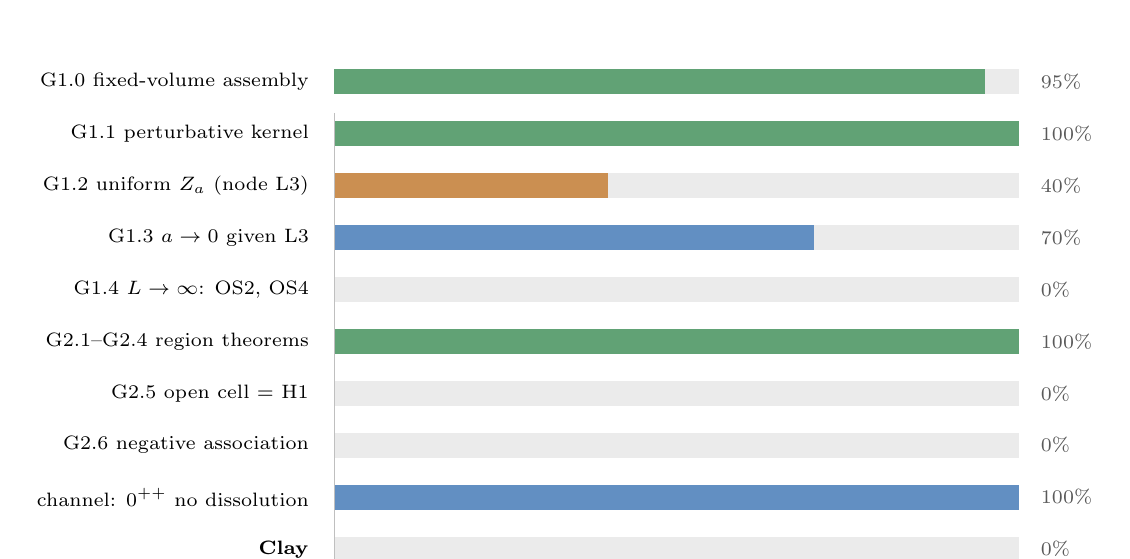
\begin{tikzpicture}[x=1cm,y=1cm,font=\scriptsize]
  \foreach \k/\nm/\pct/\cl in {%
    0/{G1.0 fixed-volume assembly}/95/cT,
    1/{G1.1 perturbative kernel}/100/cT,
    2/{G1.2 uniform $Z_a$ (node L3)}/40/cM,
    3/{G1.3 $a\to0$ given L3}/70/cC,
    4/{G1.4 $L\to\infty$: OS2, OS4}/0/cM,
    5/{G2.1--G2.4 region theorems}/100/cT,
    6/{G2.5 open cell $=$ H1}/0/cM,
    7/{G2.6 negative association}/0/cM,
    8/{channel: $0^{++}$ no dissolution}/100/cC,
    9/{\textbf{Clay}}/0/cN}{
    \pgfmathsetmacro{\yy}{-0.66*\k}
    \node[anchor=east] at (6.3,\yy) {\nm};
    \fill[black!8] (6.5,\yy-0.16) rectangle (15.2,\yy+0.16);
    \pgfmathsetmacro{\ww}{8.7*\pct/100}
    \ifnum\pct>0
      \fill[\cl!70] (6.5,\yy-0.16) rectangle ({6.5+\ww},\yy+0.16);
    \fi
    \node[anchor=west, text=black!65] at (15.35,\yy) {\pct\%};
  }
  \draw[black!25] (6.5,-0.4) -- (6.5,-6.1);
\end{tikzpicture}
\caption{Node board. Percentages are \emph{node-local} --- progress toward each node's own
goal --- and are emphatically not a percentage proof of Clay. Clay is $0\%$ because the
species is unbuilt.}
\label{fig:bars}
\end{figure}
}

% ---------------------------------------------------------------------
% Fig 5 — immune map funnel
% ---------------------------------------------------------------------
\newcommand{\figfunnel}{%
\begin{figure}[t]
\centering
\begin{tikzpicture}[x=1cm,y=1cm]
  \foreach \k/\nm in {%
    0/{positivity / analyticity-only},
    1/{cross-channel protection},
    2/{non-abelian sign calculus},
    3/{wrong half: UV control},
    4/{rename $=$ gap},
    5/{upper-bound direction},
    6/{strong-coupling only},
    7/{index $=0$},
    8/{exact reduction / duality},
    9/{constructive coercivity},
    10/{new inequality / capacity},
    11/{fixed-cell localization},
    12/{transport / monotone},
    13/{lower-bound machines},
    14/{Feshbach / Krein},
    15/{$k=0$ effective curvature},
    16/{Bethe--Salpeter two-gluon},
    17/{string tension $\to$ glueball}}{
    \pgfmathsetmacro{\yy}{-0.43*\k}
    \node[anchor=east, font=\scriptsize, text=black!75] at (6.15,\yy) {\nm};
    \draw[black!28, very thin] (6.28,\yy) -- (9.25,-3.55);
  }
  \node[fbox, text width=5.9cm, fill=cM!7, draw=cM!65] at (12.45,-3.55)
    {\textbf{ONE SPECIES}\\[2pt]
     $\operatorname{Var}_\mu(\langle v,\nabla S\rangle\mid0)\;\le\;E_\mu[H_{vv}\mid0]+W_{\mathrm{full}}-\delta$\\[2pt]
     \scriptsize uniform in $(L,U')$: this is H1 in the infrared and L3 in the ultraviolet};
\end{tikzpicture}
\caption{The immune map. Eighteen root families, spanning roughly ninety distinct routes, all
terminate at the same inequality. This is near theorem-grade \emph{exhaustiveness evidence} ---
not a theorem and not a proof, but a structural fact about where the difficulty lives.}
\label{fig:funnel}
\end{figure}
}

% ---------------------------------------------------------------------
% Fig 6 — one species, two scales
% ---------------------------------------------------------------------
\newcommand{\figscales}{%
\begin{figure}[t]
\centering
\begin{tikzpicture}[x=1cm,y=1cm]
  \node[fbox, text width=13.6cm, fill=cM!7, draw=cM!60] (species) at (7.0,4.6)
    {\textbf{One inequality: a single-sided upper bound on a conditioned variance}\\[2pt]
     \small nonperturbative \quad$\cdot$\quad non-circular \quad$\cdot$\quad free-field-failing
     \quad$\cdot$\quad $(L,a)$-uniform};
  \node[fbox, text width=5.3cm, fill=cC!8, draw=cC!50] (ir) at (3.6,1.4)
    {\textbf{Infrared face: H1}\\ $\operatorname{Var}(\xi_{k\to0})\le 1/\lambda$\\ G2's open cell \ \LM};
  \node[fbox, text width=5.3cm, fill=cC!8, draw=cC!50] (uv) at (10.4,1.4)
    {\textbf{Ultraviolet face: L3}\\ $\sup_a Z_a^{-1}\lVert H_a\rVert_D<\infty$\\ G1's open node \ \LM};
  \draw[arr] (species.south) -- (ir.north);
  \draw[arr] (species.south) -- (uv.north);
  \draw[{Stealth[length=5pt]}-{Stealth[length=5pt]}, draw=cC!60, thick, dashed]
    (ir.east) -- (uv.west);
  \node[font=\scriptsize, text=black!65] at (7.0,2.55) {same shape};
\end{tikzpicture}
\caption{The one-species reduction. The same inequality appears at two scales: as the UV
force-variance bound L3 and as the IR conditioned-variance bound H1. The shapes coincide because
$\operatorname{Var}\ge0$ can only supply a lower edge, while in
$G''=E[H]-\operatorname{Var}+W_{\mathrm{full}}$ the variance subtracts. The unification is a conjecture; the
dictionaries (Ward, residue--level-gap, $G''=E[H]-\operatorname{Var}+W_{\mathrm{full}}$) are theorems, and
building the inequality would close L3 and H1 simultaneously.}
\label{fig:scales}
\end{figure}
}

% ---------------------------------------------------------------------
% Fig 7 — numerics: curvature probe with error bars
% ---------------------------------------------------------------------
\newcommand{\figprobe}{%
\begin{figure}[t]
\centering
\begin{tikzpicture}[x=1cm,y=1cm,font=\scriptsize]
  % axes: y from -0.1 to 0.55
  \draw[arr] (0.8,-0.1*5.4-0.4) -- (0.8,0.58*5.4) ; % y axis
  \draw[arr] (0.8,-0.1*5.4-0.4) -- (9.4,-0.1*5.4-0.4) node[alab, right] {};
  \pgfmathsetmacro{\yzero}{0*5.4-0.0}
  \draw[dashed, black!50] (0.8,{0.0}) -- (9.2,{0.0});
  \node[anchor=east, text=black!60] at (0.7,0.0) {$0$};
  \node[anchor=east, text=black!60] at (0.7,{0.5*5.4}) {$0.5$};
  \node[anchor=east, text=black!55, rotate=90] at (0.15,{0.27*5.4}) {$G''$};
  % data
  \foreach \x/\val/\err/\nm in {2/0.425/0.084/{$L=4$, $k=\pi/2$},
                                4/0.307/0.055/{$L=8$, $k=\pi/4$},
                                6/0.396/0.063/{$L=8$, $k=\pi/2$},
                                8/0.319/0.005/{$W_{\rm geo}$}}{
    \pgfmathsetmacro{\ym}{(\val-\err)*5.4}
    \pgfmathsetmacro{\yp}{(\val+\err)*5.4}
    \pgfmathsetmacro{\yc}{\val*5.4}
    \draw[thick, cC!80] (\x,\ym) -- (\x,\yp);
    \draw[thick, cC!80] (\x-0.09,\ym) -- (\x+0.09,\ym);
    \draw[thick, cC!80] (\x-0.09,\yp) -- (\x+0.09,\yp);
    \fill[cC!85] (\x,\yc) circle (1.6pt);
    \node[rotate=30, anchor=north east, text=black!70, inner sep=1.5pt]
      at ({\x+0.12},-1.05) {\nm};
    \node[above=3pt, text=black!70] at (\x,{\yp+0.02}) {$\val$};
  }
\end{tikzpicture}
\caption{The $k\to0$ curvature probe on a single $L=8$ volume ($\mathrm{SU}(3)$, $\beta=5.7$),
with an $\mathrm{SU}(3)$ $L=4$ check; all plotted points are $\mathrm{SU}(3)$, while
$\mathrm{SU}(2)$ ($\beta=2.4$) reproduces the sign without being plotted. The measured points are positive and volume-stable,
and $W_{\mathrm{geo}}$ is pinned at $+0.32$. This is a $k\to0$ sign probe on a
gauge-dependent gluon mode in a flat chart, \emph{not} the gauge-invariant $0^{++}$ residue;
keeping only the proven $W_{\mathrm{geo}}\ge0$ and treating the rest statistically gives
$95\%$ one-sided lower bounds of $-0.098$ ($\mathrm{SU}(3)$) and $-0.035$ ($\mathrm{SU}(2)$),
so zero is not excluded. Label \LE.}
\label{fig:probe}
\end{figure}
}

% =====================================================================
\section{Introduction}
\label{sec:intro}
% =====================================================================

\subsection{The Clay statement, exactly}

The Clay problem, as posed by Jaffe and Witten, is:

\begin{qbox}
Prove that for any compact simple gauge group $G$, a non-trivial quantum Yang--Mills theory
exists on $\mathbb{R}^4$ and has a mass gap $\Delta>0$. Existence includes establishing
axiomatic properties at least as strong as those cited in Streater--Wightman (1964) and
Osterwalder--Schrader (1973, 1975). [Jaffe--Witten, \emph{Quantum Yang--Mills Theory}, Clay
Mathematics Institute]
\end{qbox}

Two features of this statement are habitually under-weighted and drive everything that
follows. First, it demands a \textbf{uniform} gap: not merely that each finite lattice volume
has a positive spectral gap (trivially true by compactness), but that the gap survives
$L\to\infty$ and $a\to0$ with a volume- and cutoff-uniform lower bound, and that the resulting
theory clusters exponentially at a rate $m>0$. Second, it demands that the gap be a feature of
the \textbf{gauge-invariant, physical} theory --- not of a gauge-fixed chart, and not of a
perturbative expansion around a chosen background.

The campaign's operational form of the Clay conclusion, assembled and partially
machine-verified in \code{docs/conditional-theorem.md}, is:
\begin{align*}
&\exists\,\mu\ \text{on}\ \mathbb{R}^4,\ \text{gauge-invariant, satisfying OS0--OS4};\\
&\text{non-Gaussian},\quad g_{\mathrm{ren}}/\Lambda>0;\\
&\Delta/\Lambda\ \ge\ \min(\delta_W,\delta_S)>0;\\
&|S(f\,\tau_a g)-S(f)\,S(g)|\ \le\ C\,e^{-m\|a\|},\qquad
  m\ge c\,\Delta>0,\ \ \text{all gauge-invariant local } f,g;\\
&\text{unique vacuum};\quad \text{area law } \sigma=c_\sigma\Lambda^2>0;\quad
  \text{all constants group-uniform in } (h^{\vee},\dim G,\dim\mathfrak{g}).
\end{align*}

The transfer-matrix form of the same statement is the one used throughout this paper: for the
lattice transfer matrix $T_a=e^{-H_a}$ on the gauge-invariant Hilbert space $\mathcal{H}_a$,
with vacuum $\Omega$,
\begin{equation}
\exists\,\delta>0:\qquad
\inf\operatorname{spec}\!\bigl(H_a\big|_{\Omega^\perp}\bigr)\ \ge\ \delta\Lambda
\qquad\text{for all sufficiently small } a .
\label{eq:clay-transfer}
\end{equation}

\subsection{The lock-core rewriting}

The campaign works with a sharper, channel-specific rewriting of the gap which, while not
literally equivalent to the Clay statement, is the correct object to attack. Let $\nu$ be the
Källén--Lehmann spectral measure of the gauge-invariant local operator
$O=\operatorname{tr}F^2$ (more precisely $O_S=\tfrac14\operatorname{tr}F_{\mu\nu}F^{\mu\nu}$,
the scalar density; the normalization is immaterial). Reflection positivity gives $\nu\ge0$
and $\operatorname{supp}\nu\subset[m_1^2,\infty)$, where $m_1$ is the lightest mass in the
$0^{++}$ channel. The \textbf{atom} is
\begin{equation}
f_1^2 \;:=\; \nu(\{m_1^2\}) \;=\; \bigl|\langle 0|\operatorname{tr}F^2|\mathbb{G}\rangle\bigr|^2 ,
\label{eq:atom}
\end{equation}
the squared overlap of the vacuum with the lightest $0^{++}$ glueball $\mathbb{G}$. The \textbf{lock core}
is: $f_1^2>0$ and the atom is isolated ($\Delta>0$ above it). The campaign summarises this as
\begin{equation}
\text{Clay}\iff\neg(\mathrm{iii}),\qquad
(\mathrm{iii})=\text{``the YM measure is a gapless interacting 4D CFT''.}
\label{eq:lockcore}
\end{equation}

This rewriting is useful because it names the exact analytic object (an atom weight in a
positive measure at the bottom of a channel) and the exact analytic property it has: $f_1^2$ is
\textbf{non-diagonal} (it is an off-diagonal matrix element squared),
\textbf{upper-semicontinuous} in the coupling ($\nu(\{x\})$ is usc), and requires a
\textbf{second scale} $E_2$ to certify isolation. Each of these properties will matter: usc
means continuity can only make an atom \emph{fall}, never rise; the need for $E_2$ is the
reason every bottom-functional tool is blind.

\textbf{Honesty checkpoint.} ``Clay $\iff$ atom'' is \emph{not} a theorem of equivalence. The
campaign's own adversarial audit (\code{research/unconditional/REDUCTION-AUDIT.md}) establishes
that the correct logical shape is a \textbf{diamond}, not a chain (Figure~\ref{fig:diamond}): a
gapped theory need not have an atom at all (the massive free scalar with $O={:}\varphi^2{:}$
has a gap and $f_1^2=0$), so $\text{gap}\Rightarrow\text{atom}$ is false; the true direction is
\emph{isolated atom at $\inf\operatorname{supp}\nu$ $\Rightarrow$ exponential clustering in that
channel}, conditional on that channel carrying the lightest state. This paper therefore treats
``the atom $f_1^2>0$'' as the \textbf{target object}, not as a synonym for Clay. The gap
between the two is itself a named missing step --- the ordering input that the lightest state
lies in $0^{++}$ (the corpus's \code{IN-11}, a physical input, not derivable from symmetry).

\figreduction

\subsection{The two halves}

The campaign splits Clay into two halves and a channel:

\begin{itemize}
\item \textbf{G1 (existence).} 4D continuum existence with OS axioms. The fixed-volume
  construction is essentially complete; the one genuinely open UV input is a \textbf{uniform
  renormalization constant} $Z_a$, equivalently a cutoff-uniform bound on the force Hessian
  (the node called L3). L3 is purely ultraviolet and \emph{orthogonal} to the gap --- proving it
  would make fixed-volume existence unconditional but would not help G2.
\item \textbf{G2 (gap).} The proof or transport of $f_1^2>0$ (equivalently of the coarse
  curvature $G''(0)>0$ at $k\to0$). This is where the problem lives.
\item \textbf{The physical channel.} Identifying the lightest state as $0^{++}$ and showing it
  does not dissolve (the no-dissolution theorem). This half is, conditionally, complete.
\end{itemize}

The single deepest structural finding of the campaign is that \textbf{G1's L3 and G2's H1 are
one species} (Figure~\ref{fig:scales}): both are a one-sided \emph{upper bound on a variance}.
L3 is the UV force-variance bound; H1 is the IR conditioned-variance bound
$\operatorname{Var}(\xi_{k\to0})\le1/\lambda$ (curvature form
$\operatorname{Var}_\mu(\langle v,\nabla S\rangle|0)\le E_\mu[H_{vv}|0]+W_{\mathrm{full}}-\delta$).
The shapes are
identical because $\operatorname{Var}\ge0$ can only supply a lower edge, while in the exact
identity $G''=E[H]-\operatorname{Var}+W_{\mathrm{full}}$ (with $W_{\mathrm{full}}=W_{\mathrm{geo}}+X$ as in
\S\ref{sec:wgeo}) the variance enters with a minus sign. The two faces
differ only in scale (UV versus IR). This unification is stated in the corpus as a
\textbf{structural identification and a conjecture}, not a theorem
(\code{G2-ASSEMBLE-100.md} \S7: ``a structural identification \ldots{} one closure would likely
close both faces --- but that is a conjecture, not a theorem''). This paper preserves that label.

\figscales

\subsection{What this paper is, and is not}

This paper is \textbf{not} a proof of Clay, and it contains no step labelled QED. It is:

\begin{itemize}
\item a precise statement of the reduction, with every hypothesis displayed;
\item a complete inventory of what was actually proved, labelled by type;
\item a statement of the no-gos, each with the precise reason its class fails;
\item the immune map: roughly ninety routes, each with the exact point at which it dies;
\item a specification of the missing tool: five conditions, verbatim;
\item an honest verdict.
\end{itemize}

The reader who wants only the bottom line should read \S\ref{sec:verdict}. The reader who wants
to check the work should follow the file names in \S\ref{sec:theorems}.

\subsection{Roadmap}

\S\ref{sec:halves} states the two halves and the node board with honest percentages.
\S\ref{sec:squeeze} gives the exact spectral squeeze and explains why H1 is necessary but not
sufficient. \S\ref{sec:theorems} states the proven theorems with their hypotheses.
\S\ref{sec:tools} presents the six tools and each one's free-field acid test.
\S\ref{sec:nogos} records the no-gos. \S\ref{sec:species} states the one-species reduction and
the immune map. \S\ref{sec:missing} specifies what the missing tool must satisfy.
\S\ref{sec:verdict} gives the verdict. \S\ref{sec:refs} collects verified references.

% =====================================================================
\section{The two halves: G1 (existence) and G2 (gap), and the node board}
\label{sec:halves}
% =====================================================================

\subsection{G1 --- existence}

G1 asks for a 4D continuum $\mathrm{SU}(N)$ gauge theory satisfying OS0--OS4. The campaign's
decomposition (\code{docs/PROOF-SKELETON.md} \S2) is Table~\ref{tab:g1}.

\begin{table}[t]
\centering
\begin{tabularx}{\textwidth}{@{}l>{\raggedright\arraybackslash}Xc>{\raggedright\arraybackslash}p{3.1cm}@{}}
\toprule
\textbf{Node} & \textbf{Object} & \textbf{Local \%} & \textbf{Label}\\
\midrule
G1.0 & Fixed-volume assembly: L1 definition, L2 theorem, single-block $G''\ge\delta_W$,
  GL3 compactness, GL4 reflection-positivity propagation & $\sim95\%$ (all but L3) & \LT{} mod.\ L3\\
G1.1 & Perturbative/combinatorial kernel: BRST dimension-4 classes reduce to
  $\{\operatorname{Tr}F^2,\operatorname{Tr}F\tilde F\}$; asymptotic freedom absorbs the marginal
  log; $\sum g_j^4=\zeta(4)/(16\beta_0^4)<\infty$ & 100\% & \LT{} closed\\
G1.2 & \textbf{Uniform $Z_a$ $=$ L3}: $\sup_a Z_a^{-1}\|H_a\|_D<\infty$ $=$ L2 $+$ block
  Poincaré $+$ $\Lambda_{\mathrm{UV}}$ tower uniform & $\sim40\%$ & \LM{} open\\
G1.3 & $a\to0$ continuum via OS reconstruction, given L3 & $\sim70\%$ & \LC{} on L3\\
G1.4 & $L\to\infty$, OS2 (continuous O(4)), unique vacuum OS4 (clustering) & 0\% &
  \LM{} open, entangled with G2\\
\bottomrule
\end{tabularx}
\caption{G1 node board: existence.}
\label{tab:g1}
\end{table}

The perturbative kernel G1.1 is a genuine closure: the marginal logarithm is not the obstruction
($\sum g_j^4$ converges), and the only surviving dimension-4 operators are
$\operatorname{Tr}F^2$ and $\operatorname{Tr}F\tilde F$. G1.2 is the sole open UV node, and it
is exactly a \textbf{single-sided force-variance bound} --- the same species as G2's H1. G1.3 is
conditional on G1.2 (OS0/OS1/OS3 are otherwise assembled; OS0 requires L3, OS1 and OS3 are
proved). G1.4 (OS2, infinite volume, uniqueness) is open and, crucially, \textbf{OS4 is
downstream of the gap}: a uniform gap gives clustering for free.

The campaign's honest aggregate: \textbf{G1 is 100\% assembled modulo $\{L3,G2\}$}, with 18
input rows each classified as a theorem, a reduction to L3, the gap, or the same species --- and
no genuinely independent third open item. The master document records a coarser figure of
``G1 $\approx70\%$'' (\code{docs/YANG-MILLS-MASTER.md} \S9); that number is a summary of
``perturbative kernel closed, L3 open,'' not a separate claim. We report both and do not average
them.

\subsection{G2 --- the gap}

G2 asks for $f_1^2>0$ with isolation, equivalently $G''(0)\ge\lambda$ at $k\to0$, uniform in
$(L,a)$. The decomposition (\code{research/unconditional/G2-ASSEMBLE-100.md}) is
Table~\ref{tab:g2}.

\begin{table}[t]
\centering
\begin{tabularx}{\textwidth}{@{}l>{\raggedright\arraybackslash}Xc>{\raggedright\arraybackslash}p{3.1cm}@{}}
\toprule
\textbf{Node} & \textbf{Object} & \textbf{Local \%} & \textbf{Label}\\
\midrule
G2.0 & Identity layer: $G''(k\to0)=E[H|0]-\operatorname{Var}(\nabla S|0)=V_{\mathrm{eff}}''=m_{\mathrm{eff}}^2(k\to0)$;
  exact Ward $E[a\,f]=1$; Stein/IBP $E[H]=E[f^2]$ and $E[\operatorname{Hess}V]=E[\nabla V\otimes\nabla V]\succeq0$ for every measure; $E[-D^2]=E[f^2]$ only for the free field; $G''\operatorname{Var}(\xi)=1$ iff the marginal is Gaussian; the sign sits in the \emph{conditioned} fibre Hessian (cf.\ App.~\ref{app:postaudit}) & 100\% & \LT{} identities\\
G2.1 & Haar geometric term $W_{\mathrm{geo}}=E[\Phi'']-\operatorname{Var}(\Phi')\ge0$
  (Prékopa), every mode including $k\to0$, every $L$ & 100\% & \LT\\
G2.2 & Shallow-field band $\{2g\|F\|\le N/12\}$ closed by $\Phi''\succeq N/12$
  $+$ Brascamp--Lieb & 100\% & \LT\\
G2.3 & High-field cone (WSTC): cone variance mass
  $\le(c\beta\kappa_{\max})^2e^{-c\beta(\kappa^2-\kappa_{\rm typ}^2)N_\square}\to0$,
  $L$-uniform & 100\% & \LT\\
G2.4 & AF-UV deep cone: instability $\le\mu^2e^{-c\mu^4/g^4}\to0$ & 100\% & \LT\\
\textbf{G2.5} & \textbf{Open cell $=$ typical field $\times$ high momentum}:
  the ceiling $\operatorname{Var}(\xi_{k\to0})\le1/\lambda$ (curvature form
  $\operatorname{Var}_\mu(\langle v,\nabla S\rangle|0)\le E_\mu[H_{vv}|0]+W_{\mathrm{full}}-\delta$) &
  \textbf{0\%} & \textbf{\LM{} $=$ H1}\\
\textbf{G2.6} & \textbf{Named species}: negative association / anti-FKG
  $\operatorname{Cov}(G,\Phi'|0)\le0$ & \textbf{0\%} &
  \textbf{\LM{} proven absent from nine classes}\\
\bottomrule
\end{tabularx}
\caption{G2 node board: the gap.}
\label{tab:g2}
\end{table}

The region coverage of the $(\text{field}\times\text{momentum})$ plane is about \textbf{90\%},
closed by the theorems G2.1--G2.4 (Figure~\ref{fig:plane}). The remaining one cell --- typical
field, high momentum --- is a region where all four handles fail \emph{simultaneously}: the WSTC
exponent vanishes when the field is typical, the AF-UV suppression has not begun at
$g\approx1.5$, and the $N/12$ floor is roughly ten times too small. That cell is
\textbf{exactly} $\operatorname{Var}(\xi_{k\to0})\le1/\lambda$, with zero slack. The sign --- the
actual proof --- is \textbf{0\%}.

The G2 assembly is complete in the following precise sense: of 26 input rows, every row is
either (a) a theorem or (b) a reduction to the single species; \textbf{there is no row (c)}, a
genuinely independent open item. The curvature face H1 ($G''\ge\lambda$, the \emph{inverse
zero-momentum susceptibility} $1/\chi$) and the spectral-edge face $H^*$ ($f_1^2\ge r_0$ with
isolation I2) are \emph{not} one object: by the squeeze $f_1^2/\chi\le m_1^2\le M_0/\chi$, H1 is a
susceptibility that \emph{upper}-bounds $m_1^2$ and is necessary but strictly weaker. The
identification $H^*=\text{H1}$ is not merely unproved but is \emph{contradicted} for composite
operators --- the free massive $\mathord{:}\varphi^2\mathord{:}$ has a gap ($m_1=2m$) yet
$G''=1/\chi\ne m_1^2$ --- and every gauge-invariant Yang--Mills operator is composite. The gap is
$H^*$; the rigorous content is the residue--level-gap lemma and the exact Ward identity $E[a\,f]=1$.

\figplane

\subsection{The dimensional correction}

One correction must be recorded because it is easy to get wrong and it changes what
``$G''\ge\lambda$'' means (\code{docs/PROOF-SKELETON.md}, G1-CONTINUUM-SCALING). For the
dimensionless Wilson action, the Hessian satisfies
\begin{equation}
G''_a=a^2\,m_{\mathrm{phys}}^2,\qquad
m_{\mathrm{lat}}=\sqrt{G''_a}=a\,m_{\mathrm{phys}},\qquad
\Delta=\lim m_{\mathrm{lat}}/a .
\label{eq:dim}
\end{equation}
Therefore a claim of the form ``at fixed $a$, $G''_a\ge\lambda$ with $\lambda$ a positive
\emph{constant}'' is dimensionally wrong for the gap: it would give
$m_{\mathrm{phys}}=\lim\sqrt{\lambda}/a=+\infty$, the free-box UV scale, a lattice artifact
rather than a particle. The correct target is a \textbf{ratio} $G''_a/a^2\ge\Delta_0^2$ at the
asymptotically-free scaling rate, i.e.\ $\lambda_a\sim a^2\Delta_0^2$, with $\lambda_a$
transported multiplicatively by $Z_O^2$. The transport itself is free (it is a square); what is
not free is the non-zero seed it multiplies. This distinction pervades the honest reading of the
numerics in \S\ref{sec:tools} and \S\ref{sec:verdict}.

\subsection{The node board, in one table}

\begin{table}[t]
\centering
\begin{tabularx}{\textwidth}{@{}ll>{\raggedright\arraybackslash}p{4.4cm}
  >{\raggedright\arraybackslash}X@{}}
\toprule
\textbf{Half} & \textbf{Object} & \textbf{Local completion} & \textbf{Status}\\
\midrule
G1 & 4D continuum existence & 100\% assembly modulo $\{L3,G2\}$ & \LT{}+\LC, one UV node open\\
G1.2 & UV uniform $Z_a$ $=$ L3 & $\sim40\%$ & \LM\\
G2 & Gap: region coverage & $\sim90\%$ & theorems G2.1--4\\
G2.5--6 & Gap: sign / proof & \textbf{0\%} & \LM{} $=$ H1, the species\\
Channel & $0^{++}$ identification $+$ no dissolution & 100\% & \LC\\
\textbf{Clay} & existence $\wedge$ gap & \textbf{0\%} & \textbf{open}\\
\bottomrule
\end{tabularx}
\caption{The node board in one table (see also Figure~\ref{fig:bars}).}
\label{tab:nodes}
\end{table}

The percentages are \textbf{node-local} --- progress toward each node's own goal --- and are
emphatically \textbf{not} a percentage proof of Clay. Clay is 0\% because the species is
unbuilt.

\figbars

% =====================================================================
\section{The exact spectral squeeze, and why H1 is necessary but not sufficient}
\label{sec:squeeze}
% =====================================================================

\subsection{Setup}

Let $\nu\ge0$ be the Källén--Lehmann measure of $\operatorname{tr}F^2$, with
$\operatorname{supp}\nu\subset[m_1^2,\infty)$, atom weight $f_1^2=\nu(\{m_1^2\})$, and moments
$M_k=\int s^k\,d\nu(s)$. Let $a$ be the zero-momentum coarse mode
($a=\langle v,\log U\rangle$ for the relevant mode; $\operatorname{Var}(a)$ is the
zero-momentum connected propagator). The \textbf{susceptibility} is
\begin{equation}
\chi \;:=\; \operatorname{Var}(a) \;=\; \int s^{-1}\,d\nu(s)
\qquad(\text{the zero-momentum connected two-point function}).
\label{eq:chi}
\end{equation}
This is the inverse of the effective curvature only in the Gaussian case; in general it is a
residue-weighted \emph{harmonic} mean of the masses, dominated by the lightest residue. It is
not the lightest mass.

\subsection{The squeeze \LT}

For any such $\nu$:
\begin{equation}
\frac{f_1^2}{\chi}\ \le\ \inf\operatorname{supp}\nu\ \le\ \frac{M_0}{\chi}.
\label{eq:squeeze}
\end{equation}
\begin{proofx}
\textbf{Lower inequality.} $\chi m_1^2=f_1^2+m_1^2\int_{s>m_1^2}s^{-1}d\nu(s)\ge f_1^2$, since
$m_1^2s^{-1}\ge1$ on the support above $m_1^2$. Hence $m_1^2\ge f_1^2/\chi$.
\textbf{Upper inequality.} On $\operatorname{supp}\nu$, $s\ge m_1^2$, so $s^{-1}\le m_1^{-2}$,
hence $\chi=\int s^{-1}d\nu\le M_0/m_1^2$, i.e.\ $m_1^2\le M_0/\chi$.
\end{proofx}

Both inequalities are elementary and exact. They are the entire content of the ``squeeze'' and
they contain no dynamical input.

\subsection{H1 is necessary, not sufficient}

The condition H1 is
\begin{equation}
\mathrm{H1}:\qquad \operatorname{Var}_\mu(a_{k\to0})=\chi\ \le\ 1/\lambda,
\qquad\text{uniform in }(L,a).
\label{eq:h1}
\end{equation}

\textbf{Necessity.} If the theory has a gap $m_1\ge\sqrt\lambda$ (with the normalization $M_0$
fixed), then $\chi=\int s^{-1}d\nu\le M_0/\lambda$, so $\chi\le M_0/\lambda$. This is a
theorem: $\text{gap}\Rightarrow\chi\le M_0/\lambda$ (up to the normalization constant). The
corpus records it as $\chi=\int s^{-1}d\nu\le M_0/\lambda$ (\code{REDUCTION-AUDIT.md}).

\textbf{Non-sufficiency.} Take (Figure~\ref{fig:measure}, right panel)
\begin{equation}
\nu=w\,\delta_\varepsilon+(1-w)\,\delta_S,\qquad w/\varepsilon\le1/\lambda .
\label{eq:thinatom}
\end{equation}
Then $\chi=w/\varepsilon+(1-w)/S<\infty$, so H1 holds, while
$\inf\operatorname{supp}\nu=\varepsilon\to0$. \textbf{H1 holds and the gap fails.} The measure
has a thin atom at $\varepsilon$, invisible to the susceptibility because the susceptibility is
a harmonic mean: a tiny residue at tiny mass contributes $w/\varepsilon$, which can be kept
below $1/\lambda$ by taking $w$ small. The susceptibility sees the \emph{residue-weighted}
mass, not the lightest mass.

This counterexample is not a pathology; it is the exact obstruction the campaign met
everywhere. It is why the audit's verdict is that the chain written as $\iff$ is unsound: read
against the corpus's own definitions, it is \textbf{(iv) false $\to$ (iii) conjecture $\to$
(ii) definition}, plus one genuine one-directional theorem. The final $\iff$ (H1 $\iff$ gap)
holds in one direction only.

\subsection{The correct sufficient condition}

The repair is the pair:
\begin{equation}
(f_1^2\ge r_0)\ \wedge\ (\chi\le1/\lambda)
\qquad\Longrightarrow\qquad
m_1^2\ \ge\ f_1^2/\chi\ \ge\ r_0\lambda\ >\ 0 .
\label{eq:sufficient}
\end{equation}
This is immediate from the squeeze and it is the campaign's central logical content: \textbf{a
lower bound on the mass needs both a residue floor and a susceptibility ceiling.} The residue
floor is the hard half; the susceptibility ceiling is H1. The campaign's honest statement of the
missing input is therefore not H1 alone but
\begin{equation}
H^*:\qquad f_1^2\ge r_0>0\ \ \text{with isolation } I_2,
\qquad(\text{and }\chi\le1/\lambda\text{ as the matching ceiling}),
\label{eq:hstar}
\end{equation}
where $I_2$ is $\Lambda:=\inf\operatorname{supp}(\nu-f_1^2\delta_{m_1^2})$,
$\Lambda-m_1^2\ge\delta>0$. The residue--level-gap lemma (\S\ref{sec:reslevel}) turns I1 into
I2 and back, so $H^*=\text{H1}$ \emph{as a structural identification}; but the identification is
the conjecture, and the residue datum is strictly stronger than the bare gap.

\subsection{Why H1 is blind: Schur concavity}

H1 is an \textbf{upper-only} condition. Every functional of $\nu$ built from its moments or from
positivity is a Schur-concave functional of the measure, hence gives an \textbf{upper} bound on
the atom weight, never a lower bound. Concretely, for any nonnegative test function $\varphi$,
\begin{equation}
f_1^2\ \le\ M_0,\qquad f_1^2\ \le\ \chi m_1^2 ,
\label{eq:schur}
\end{equation}
and the first is the trivial ``atom $\le$ total mass,'' the second the squeeze. There is no
positivity-only route to a \emph{lower} bound on $f_1^2$: the free massless field is a
legitimate OS theory with $\nu$ supported on $[0,\infty)$ and $f_1^2=0$, and any positivity
argument that would force $f_1^2>0$ must also force it for the free field, which is false. This
is the master obstruction (\S\ref{sec:schur}), and it is why H1 --- a second-moment inequality
--- is structurally blind to the light state that the squeeze's counterexample exploits.

\subsection{$G''$ versus $1/\chi$}

The curvature $G''=V_{\mathrm{eff}}''$ and the inverse susceptibility $1/\chi$ coincide only for
a Gaussian marginal. Ward's identity
\begin{equation}
G''\cdot\operatorname{Var}(a)=1
\qquad\iff\qquad
\text{the marginal of } a \text{ is Gaussian},
\label{eq:ward}
\end{equation}
is exact in one direction only. Measured at $\beta=2.5$, the two differ by $2$--$5\%$
($G''\approx0.281$ versus $1/\operatorname{Var}\approx0.272$; \code{FORGE5-SL-IR-SINGLE.md},
quoted in \code{docs/new-tools-registry.md}). So even the ``curvature face'' is not literally
the susceptibility; it is a second-moment object that equals the susceptibility only in the
Gaussian limit. The unification $G''=1/\chi=\text{H1}$ is therefore a \emph{conjecture with a
measured $2$--$5\%$ gap}, not an identity. The exact identity that does hold is the variance
decomposition of \S\ref{sec:feshbach}.

\subsection{The verdict on the reduction}

The honest logical skeleton (\code{REDUCTION-AUDIT.md} \S``What actually survives'',
Figure~\ref{fig:diamond}) is:

\begin{itemize}
\item \LT{} isolated atom at $\inf\operatorname{supp}\nu$ of a channel $\Rightarrow$ exponential
  clustering in that channel;
\item \LT{} $\text{gap}\Rightarrow\chi\le M_0/\lambda$;
\item \LT{} $G''\ge\lambda\Rightarrow\operatorname{Var}(a)\le1/\lambda$ (Brascamp--Lieb, one way);
\item \LC{} the unification $H^*=\text{H1}$ (``one object'') --- a structural identification,
  not a theorem;
\item \textbf{(iv) false} $\text{gap}\iff\text{atom}$, and $\text{H1}\iff\text{gap}$.
\end{itemize}

Written as $\iff$, the chain is unsound. Its true shape is a \textbf{diamond of implications
converging on the necessary condition $\chi\le1/\lambda$}, with the sufficient condition being
the strictly stronger $H^*=\text{I1}\wedge\text{I2}$. Proving H1 alone does not yield the gap
(the tiny-residue counterexample); proving $H^*$ does, but $H^*$ is not H1. This is the first
place where the campaign's honesty line is load-bearing, and we state it plainly: \textbf{the
reduction relocates the residue content; it does not remove it.}

% =====================================================================
\section{Proven theorems}
\label{sec:theorems}
% =====================================================================

This section states each theorem with its precise hypothesis and label. Every theorem names the
file containing the proof. We separate the unconditional strong-coupling results from the
conditional ones and state explicitly, where relevant, that a residue theorem is \textbf{not} a
gap theorem.

\subsection{The strong-coupling residue theorem (P3) --- \LT, regime-limited, I1 only}

\src{\code{research/unconditional/PROOF-P3-UNCONDITIONAL.md}; \code{PROOF-P1P2.md};
\code{PROOF-P3.md}.}

\begin{claimbox}{cT}
\claimhead{Theorem}{(P3)} \emph{Fix $a>0$. There exist $\beta_1=\min(1/48,c/N)>0$ and, for
each $\beta<\beta_1$, a constant $r_0(\beta)=\tfrac12 c_1(\beta)u(\beta)^p>0$ ($c_1$ a positive
$\mathrm{SU}(N)$ group constant, $u(\beta)$ the fundamental character coefficient,
$u\asymp\beta$), such that for every torus $T^4_L$,}
\begin{equation}
f_{1,L}^2=\lim_{t\to\infty}e^{m_1(L)t}\,C_L(t)\ \ge\ r_0(\beta)\ >\ 0,
\label{eq:p3}
\end{equation}
\emph{\textbf{uniformly in $L$}.}

\smallskip
\textbf{Hypotheses and imports.} Wilson action $S=\beta\sum_p\bigl(1-N^{-1}\operatorname{Re}
\operatorname{tr}U_p\bigr)$, Haar measure, character expansion with $c_r(\beta)\ge0$. The proof
imports the Osterwalder--Seiler connected-composite expansion and the Kotecký--Preiss criterion;
the single lemma left as ``standard assembly'' by the earlier drafts --- the \textbf{graded-strip
Kotecký--Preiss lemma} --- is written out in full in \code{PROOF-P3-UNCONDITIONAL.md} \S2--\S4.
Its hypothesis is the per-site condition $u(\beta)K<1$ with explicit $K\le CN$ (the plaquette
adjacency degree is $\le12$; the $\mathrm{SU}(N)$ link multiplicity is polynomial in $N$,
bounded by $CN$ on the fundamental sector). The one constant not reduced to a decimal is the
constant in $C_g\le CN$; its \emph{existence} is proved, and its value only shifts the prefactor
of $\beta_1$.

\smallskip
\textbf{Proof skeleton.} (i) $\operatorname{tr}F^2$ is a finite A1g sum of local plaquette
observables, so $C(t)$ is a sum over connected polymers; absolute convergence is the KP
condition $uK<1$, uniform in volume and strip length. (ii) A connected polymer linking time $0$
to time $t$ must meet every intermediate slice, so its plaquette cost is $\ge t/a$; equality
forces a single fundamental flux tube, weight $a_0u^{t/a}=a_0e^{-m_1t}$. This tube is the
\emph{unique} leading concentration, and its amplitude $a_0(\beta)>0$ is a product of positive
fundamental character coefficients times the positive singlet recoupling
$f\otimes\bar f\to1$. (iii) $f_1^2=|\langle\Omega|O|G\rangle|^2$ is a modulus-square, so no sign
can undo it. (iv) Every non-tube polymer costs a whole factor $u$ more; the KP criterion is
independent of backbone length, so the remainder is $O(u)$ uniformly in $t,V,L$.

\smallskip
\textbf{What it is.} A genuine \textbf{volume- and $L$-uniform lower bound on the residue}
$f_1^2$ at strong coupling, fixed $a$. It is the half that Shen--Zhu--Zhu does not supply: SZZ
gives a gap (a decay-rate \emph{upper} bound), P3 gives a residue \emph{lower} bound.

\smallskip
\textbf{What it is not --- the correction that must be preserved.} Earlier drafts claimed the
integer cost grading ``additionally yields I2 (isolation).'' \textbf{That claim is wrong} and is
corrected in \code{PROOF-P3-UNCONDITIONAL.md} \S5 and \code{PROOF-P1P2.md} \S3. The cost grading
grades \textbf{polymer amplitudes}, not \textbf{transfer-matrix eigenvalue spacing}. It makes
the single tube the unique leading term (I1), but the KP/OS remainder is a $t$-uniform $O(u)$,
never an $O(e^{-\delta t})$; so it cannot separate a second atom from one at $\varepsilon\to0$,
nor place the excited $0^{++*}$ (at $\approx1.5\,m_1$) below the $2m_1$ continuum. \textbf{I2
remains exactly the open step.} Hence P3 is a \textbf{residue theorem, not a gap theorem.} The
strong-coupling gap itself is classical Osterwalder--Seiler (1978) and is not what P3 proves.

\smallskip
\textbf{Scope.} Fixed $a$; $\beta<1/48$; no continuum limit $a\to0$; no transport to
$\beta\approx2.5$. The analyticity radius $1/48$ is the Ursell series radius, not a wall in the
spectrum: the residue $f_1^2(\beta)=|a(\beta)|^2$ is real-analytic wherever $\lambda_1$ is
simple and isolated (Kato; analytic in a disk), so $1/48$ is a limitation of the \emph{method},
not of the object. But the method stops there, and no absolute strong-coupling method can cross
its analyticity radius.
\end{claimbox}

\subsection{The no-dissolution kinematic theorem --- \LC}
\label{sec:nodiss}

\src{\code{research/unconditional/PROOF-NO-DISSOLUTION-KINEMATIC.md};
\code{PROOF-DISSOLUTION-SPECTRAL-DENSITY.md}.}

\begin{claimbox}{cC}
\claimhead{Theorem}{(no dissolution)} \emph{Suppose (K-A) the theory has a uniform gap
$m_g\ge\mu>0$, and (K-B) the lightest $0^{++}$ satisfies $m_{0^{++}}<2m_{\mathrm{lightest}}$
(implied by $0^{++}$ being the overall lightest). Then the lightest $0^{++}$ is an isolated atom
of its channel, separated from every continuum by a margin equal to its own mass:
$m_{0^{++}}<\theta_{0^{++}}=2m_g$.}

\smallskip
\textbf{Proof skeleton.} In the confined phase there is no asymptotic gluon, hence no $(gg)$
cut; the lowest continuum in the $0^{++}$ channel is two glueballs, at $\theta\ge2m_g$. If the
$0^{++}$ is the overall lightest, $m_{0^{++}}=m_g$, so $m_{0^{++}}<2m_{0^{++}}\le\theta$. The
atom sits strictly below every continuum by its own mass. Dissolution would require a continuum
at or below $m_{0^{++}}$, i.e.\ a state lighter than $\tfrac12m_{0^{++}}$ --- a level crossing
\textbf{from below} --- or gap closure. Same-channel $0^{++}$ versus excited $0^{++*}$ is a von
Neumann--Wigner avoided crossing (order cannot flip); a cross-channel $\{0^{++},2^{++}\}$
ordering flip is a relabeling (residues unchanged), and true dissolution needs the factor-2
hierarchy $m_{0^{++}}\ge2m_{\mathrm{lightest}}$.

\smallskip
\textbf{Sharpening.} In $0^{++}$, charge conjugation $C$ and parity $P$ cannot separate $gg$
from $(gg)(gg)$ (both are $C$-even, $P$-even), so the \emph{operative} threshold $\Lambda$ for
isolation is the excited $0^{++*}$ at $\approx1.5\,m_g$ (physically $1.56\,m_{0^{++}}$), not the
two-glueball $2m_{0^{++}}$. The coarser target ``no $0^{++}$ below $2m_g$'' is false; the correct
I2 is a gap to the excited glueball of size $\delta\approx0.5\,m_1$, fixed by power counting, not
symmetry (\code{PROOF-ISOLATION.md} \S4; \code{PROOF-EDGE-E2.md}).

\smallskip
\textbf{Conditional.} The theorem is a genuine kinematic theorem but inherits rather than proves
its antecedents: (K-A) is the gap, and (K-B) is the ordering input (\code{IN-11}). It fails only
on gap closure (deconfinement, not the zero-temperature smooth crossover) or on a factor-2
hierarchy. Both are dynamics, neither a smooth-crossover effect. The result is therefore \LC: it
converts ``is the $0^{++}$ an atom?'' into ``is it below the two-body threshold?'' --- and the
antecedent is exactly the open dynamics.
\end{claimbox}

\subsection{Non-negativity of the Haar geometric curvature --- \LT}

\src{\code{research/unconditional/PROOF-JACOBIAN-SAVES.md}.}

\begin{claimbox}{cT}
\claimhead{Theorem}{($W_{\mathrm{geo}}\ge0$)} \emph{Work in the flat chart
$X_\ell=\log U_\ell\in\mathfrak{su}(N)$, so Haar is $dU=J\,dX$ with $\Phi=-\log J$. For
$\mathrm{SU}(N)$, $\Phi=\sum_{i<j}g(\lambda_i-\lambda_j)$ with
$g(d)=-2\log\bigl(\sin(d/2)/(d/2)\bigr)$; on $|d|<2\pi$, $g''\ge1/6$. Hence $\Phi$ is convex,
$e^{-\Phi}dX$ is log-concave, and by Prékopa every linear marginal $a=\langle v,\log U\rangle$
has convex free energy:}
\begin{equation}
W_{\mathrm{geo}}:=E[\Phi'']-\operatorname{Var}(\Phi')\ \ge\ 0
\qquad\text{for every mode, every } k \text{ including } k\to0,\text{ uniformly in } L.
\label{eq:wgeo}
\end{equation}
\emph{Additionally, pointwise, $\Phi''\succeq0$ under any measure and any $\beta$, giving
Lemma B: $E[\Phi''|0]\ge(N/12)\|v\|^2$ ($\mathrm{SU}(2)$: $1/6$; $\mathrm{SU}(3)$: $1/4$;
measured $0.34$, $0.46$). At $\beta=0$ the geometric term is the whole curvature: $\mathrm{SU}(2)$
$V_{\mathrm{eff}}''=0.248$ versus $E[\Phi'']-\operatorname{Var}(\Phi')=0.246$, an exact
closure.}

\smallskip
\textbf{The exact split and what fails.} The identity is
\begin{equation}
\begin{aligned}
G''(0)&=E\bigl[H_{vv}+\Phi''\,\big|\,a=0\bigr]
        -\operatorname{Var}\bigl(G_v+\Phi'\,\big|\,a=0\bigr)
        =\Delta_{\mathrm{dyn}}+W_{\mathrm{geo}}+X,\\
\Delta_{\mathrm{dyn}}&=E[H]-\operatorname{Var}(G),\qquad
X=-2\operatorname{Cov}(G,\Phi').
\end{aligned}
\label{eq:split}
\end{equation}
$W_{\mathrm{geo}}$ is the curvature of the pure-Haar marginal; $X$ is the cross-fluctuation of
the action force with the Jacobian. The theorem bounds $W_{\mathrm{geo}}$ from \textbf{below by
0}, but the \emph{measured} $W_{\mathrm{geo}}\approx+0.32$ is what carries the sign at
$\beta=2.5$. Certifying $W>\operatorname{Var}-E[H]$ needs an upper bound on
$\operatorname{Var}(G|0)$, which is precisely the induced-mass/H1 object. So this is a
\textbf{sign theorem, value-free}, not a gap theorem. The $-0.165$ ``DEAD-lean'' value reported
elsewhere is a proxy that dropped exactly $+W$; measured exactly on its own mode, the marginal
is $+0.51$ (\S\ref{sec:tools}).
\end{claimbox}

\subsection{Gauge-invariant Perron--Frobenius --- \LT{} finite volume, plus an edge no-go}

\src{\code{research/unconditional/PROOF-GAUSS-INVARIANT-PF.md}.}

\begin{claimbox}{cT}
\claimhead{Theorem}{(gauge-invariant PF)} \emph{On a finite lattice, $\beta>0$, the transfer
matrix $T=e^{-aH}$ has a strictly positive kernel $T(U,V)>0$ for all $U,V$ (a limit of the
electric heat kernel, which is positive by
$K_t(g,h)=\sum_\lambda d_\lambda\chi_\lambda(g^{-1}h)e^{-tC_\lambda}>0$, times a positive
magnetic weight). Since $T(gU,gV)=T(U,V)$, it descends to a strictly positive kernel
$\bar T$ on $\mathcal{A}/\mathcal{G}$; for $0\le f\in H_{\mathrm{phys}}$, $f\ne0$,
$(Tf)(U)>0$ everywhere. So $T$ is positivity-improving at every $\beta>0$, and by
Jentzsch/Krein--Rutman $\lambda_0=1$ is simple with a strictly positive vacuum $\Omega\equiv1$,
and $0\le\lambda_1<\lambda_0$, giving a finite-volume gap
$\Delta_V=-(1/a)\log\lambda_1>0$.}

\smallskip
\textbf{Why this is honest and why it falls short.} The proof uses the \textbf{full positive
Haar measure}, no gauge slice, so no Gribov copy or Faddeev--Popov sign enters --- the honest
content of ``a positivity gauge-fixed PF lacked.'' But (i) $\lambda_1$ is the lightest state
over \emph{all} channels, not the $0^{++}$ specifically; (ii) $\inf_V\Delta_V>0$ is the mass gap
and is not obtained --- PF/Dobrushin constants scale like $e^{-cV}$, so finite-volume gaps are
\emph{upper} bounds on $\Delta_{\mathbb{R}^4}$; (iii) at $a\to0$ compactness fails, and the free
field (reflection-positive, PF, strictly positive vacuum) has $\Delta_V\to0$.

\smallskip
\textbf{The exact edge obstruction \LN.} The vacuum is $0^{++}$ and the lightest scalar
glueball is \emph{also} $0^{++}$: they share the channel. The $0^{++}$-projected transfer matrix
is still positivity-improving, so its Perron vector is the \textbf{vacuum} (top of the sector)
and the glueball is the second state, in $\Omega^\perp\cap(0^{++})$ --- exactly where the single
reflection-positivity cone degenerates. To reach the glueball one would need a second invariant
cone / total positivity (a Karlin flag) on $\mathcal{A}/\mathcal{G}$, but the quotient carries
\textbf{no order}, so no Gantmacher--Krein/TP cone exists. Gauge invariance reaches the vacuum
and the gap, never the glueball. The decisive check is on the physical space itself: free
Maxwell is PF and strictly positive with a finite-volume gap, yet its $0^{++}$ spectrum is a
two-photon cut from zero, $f_1^2=\nu(\{0\})=0$. Gauge-invariant PF plus strict positivity plus a
finite-volume gap \textbf{does not imply} a glueball atom.
\end{claimbox}

\subsection{The strong-coupling coarse Poincaré lemma (Lemma SC) --- \LT, regime-limited}

\src{\code{research/unconditional/PROOF-COARSE-POINCARE.md} \S(c).}

\begin{claimbox}{cT}
\claimhead{Lemma}{(SC)} \emph{At $\beta<1/48$, Shen--Zhu--Zhu give a uniform LSI
$\operatorname{Var}_\mu(F)\le(1/\lambda_\mu)\int|\nabla F|^2d\mu$, uniformly in volume. For a
block averaging map $P$ with $\operatorname{Lip}(P)=C_{\mathrm{blk}}=O(1)$ (averaging is a
contraction, volume-independent), set $F=\varphi\circ P$. Then for the pushed-forward measure
$\nu=P_*\mu$,}
\begin{equation}
\operatorname{Var}_\nu(\varphi)\ \le\ \frac{C_{\mathrm{blk}}^2}{\lambda_\mu}
\int|\nabla\varphi|^2\,d\nu ,
\label{eq:sc}
\end{equation}
\emph{uniformly in $(L,a)$. So the coarse Poincaré inequality holds at strong coupling with
$\lambda=C_{\mathrm{blk}}^{-2}\lambda_\mu$.}

\smallskip
\textbf{Scope.} This is a genuine anchor, but it lives exactly where the full LSI already
holds. It does not transport to $\beta=2.5$, which lies outside every high-temperature regime.
The file's three direct routes to $\beta=2.5$ fail for independent, nameable reasons: the
effective action is Savvidy-indefinite (not provably convex; the bare coarse Hessian minimum is
$\approx-0.3$, and the one-loop Schur form is undefined because $H_{ff}$ is indefinite); the
block gap is a \emph{fast} relaxation rate, not the slow stiffness, and the only variance bound
runs the wrong way by $\approx e^{5N_p}$; and the provable regime is $\beta<1/48$.
\end{claimbox}

\subsection{The Feshbach--Bogoliubov two-block lemma and the exact variance decomposition ---
\LT{} abstract / identity}
\label{sec:feshbach}

\src{\code{research/unconditional/FORGE-BLIND.md} \S2; \code{INVENT-VARIANCE-INEQ.md};
\code{docs/new-tools-registry.md} A2.}

\begin{claimbox}{cT}
\claimhead{Lemma}{(two-block gap; unconditional, abstract)} \emph{Let}
\begin{equation}
A=\begin{pmatrix} A & B\\ B^* & C\end{pmatrix}
\quad\text{on}\quad \mathcal{H}=\mathcal{H}_-\oplus\mathcal{H}_+,
\qquad C\ge\gamma I .
\label{eq:twoblock}
\end{equation}
\emph{Define the Schur complement $S:=A-BC^{-1}B^*$ on $\mathcal{H}_-$. If $S\ge\mu I$, then}
\begin{equation}
A\ \ge\ \min\Bigl\{\frac{\mu}{1+2\|B\|^2/\gamma^2},\ \frac{\gamma}{2}\Bigr\}\cdot I\ >\ 0 .
\label{eq:twoblock-bound}
\end{equation}
\begin{proofx}
$\langle u,Au\rangle=\langle u_1,Su_1\rangle+\gamma\|u_2+\gamma^{-1}B^*u_1\|^2$; put
$v_2=u_2+\gamma^{-1}B^*u_1$ and use
$\|u_2\|^2\le2\|v_2\|^2+2\|B\|^2\gamma^{-2}\|u_1\|^2$.
\end{proofx}

The lemma needs \textbf{no hypothesis of a positive Hessian}; $A$ may be arbitrarily negative.
The indefinite Savvidy Hessian is not hidden but \emph{converted} into the demand $S\ge\mu>0$.
For 4D pure $\mathrm{SU}(N)$, this becomes the \textbf{tachyonic-compensation inequality} (TCI):
\begin{equation}
\langle\varphi,Q\varphi\rangle+\langle\varphi,K\varphi\rangle-cF\ \ge\ \mu>0
\qquad\text{for all }\|\varphi\|=1,\ \varphi\in\mathcal{H}_- ,
\label{eq:tci}
\end{equation}
i.e.\ the gauge-invariant effective potential is convex at its minimum, pointwise and
nonperturbatively, and the Savvidy vacuum has no imaginary part. The tool is not vacuous: on the
free massless field, $Q=0$, the bottom of $A|_-$ is $0$, $S$ is not $\ge\mu$, TCI fails, and the
certificate correctly returns $0$.

\smallskip
\textbf{Lemma NS (eliminating a negative block raises the survivor).} In the quadratic form
$\begin{psmallmatrix}A&B\\B^*&C\end{psmallmatrix}$ with $C\prec0$, the Schur complement satisfies
$\Sigma=A-BC^{-1}B^*=A+B|C|^{-1}B^*\succeq A$. This is true and is a genuine gain, but it
certifies only the \textbf{fast} half of the block BBS scheme; the slow wall is the variance
term, which the block elimination never touches
(\code{D-BBS-INTEGRATE-NEG.md}).

\smallskip
\textbf{Exact variance decomposition (Savvidy-corrected Brascamp--Lieb).} With
$K=\Pi_0\operatorname{Hess}V\,\Pi_0$, $c=\Pi_0\operatorname{Hess}V\,v$,
$h_n=v^{\mathsf T}\operatorname{Hess}V\,v$,
\begin{equation}
\begin{aligned}
G''(0)&=S(v)-D(v),\\
S&=E_\mu\bigl[h_n-\langle K^{-1}c,c\rangle\mid0\bigr],\qquad
D=\operatorname{Var}_\mu(\partial_nV\mid0)-E_\mu\bigl[\langle K^{-1}c,c\rangle\mid0\bigr].
\end{aligned}
\label{eq:vardecomp}
\end{equation}
Sign law: $D\le0\iff K\succeq0$ (true BL); $D=0\iff$ Gaussian; $D>0\iff$ fiber Savvidy. At
$\beta=0$, $V=\Phi$ is convex, so $D\le0$ and $G''\ge S\ge N/12>0$ --- a theorem. At
$\beta=2.5$, $D/S\approx2\%$ (measured; the marginal is essentially Gaussian), so $G''>0$ is
numerically robust with $\sim98\%$ margin. The residual is a uniform bound on the $2\%$ fiber
defect, which is H1. The acid test is non-trivial: the free Gaussian has $D=0$, and the $k\to0$
mode has $\operatorname{Var}(a)=\infty$, so $S=0$ and $G''=0-0=0$; the tool manufactures no
false positivity.
\end{claimbox}

\subsection{The residue--level-gap lemma and the conditional theorem --- \LT{} / \LC}
\label{sec:reslevel}

\src{\code{GAP-G2-edge} (quoted in \code{G2-ASSEMBLE-100.md} \S2);
\code{docs/conditional-theorem.md}.}

\begin{claimbox}{cT}
\claimhead{Lemma}{(residue--level-gap)} \emph{Let
$\Lambda:=\inf\operatorname{supp}(\nu-f_1^2\delta_{m_1^2})$. Then}
\begin{equation}
f_1^2\ \ge\ \frac{\Lambda M_0-M_1}{\Lambda-m_1^2}
= M_0\,\frac{\Lambda-\bar R}{\Lambda-m_1^2},
\qquad \bar R:=\frac{M_1}{M_0}.
\label{eq:reslevel}
\end{equation}
\emph{The right side is positive \textbf{iff} $\Lambda>\bar R$, and $\Lambda>\bar R$ suffices
(if $f_1^2=0$ then $\Lambda=m_1^2$ and $\bar R\ge\Lambda$). The converse fails (a positive atom
with a heavy tail can have $\bar R>\Lambda$). So this is a self-certifying sufficient
certificate, not an equivalence. By this lemma and Theorem A of \code{mass-spectrum},
$\text{atom(I1)}\wedge\text{I2}\iff$ sharp two-exponential decay
$C(t)=f_1^2e^{-m_1t}(1+\eta(t))$, $|\eta(t)|\le Be^{-\delta t}$.}

\smallskip
\textbf{The conditional theorem.} Under the twelve named inputs \code{IN-0} \ldots{} \code{IN-11}
(\code{docs/conditional-theorem.md}), there exists a gauge-invariant measure $\mu$ on
$\mathbb{R}^4$ satisfying OS0--OS4, non-Gaussian with $g_{\mathrm{ren}}/\Lambda>0$, with
$\Delta/\Lambda\ge\min(\delta_W,\delta_S)>0$, unique vacuum, area law, and group-uniform
constants; and the gap is equivalent to
$\inf\operatorname{spec}(H_a|_{\Omega^\perp})\ge\delta\Lambda$ uniformly in $a$. The synthesis
chain is \textbf{9/9 closed} (each gluing lemma is either proved or reduced to a named input),
and the core of S3, S4, S5, S10, S11 is machine-verified in Lean with frozen axioms
(\code{Handoff.lean}, \code{RGHandoff.lean}, \code{HandoffMargin.lean},
\code{GlueA.spectral\_decay}, \code{GL2a.lean}, \code{GL2bPrime.lean}, \code{GL7Dual.lean},
\code{GroupUniform.lean}, \code{GL6Fubini.lean}, \code{Conditional.lean}; the checks are listed
in \code{conditional-theorem.md} \S6).

\smallskip
\textbf{Honest status of the inputs.} Twelve inputs: two proved or machine-verified
(\code{IN-1} bounded class, vacuous, and \code{IN-8} assembly), seven open (\code{IN-2},
\code{IN-3}, the 4D part of \code{IN-4}, \code{IN-5}, \code{IN-6}, the quantitative constants of
\code{IN-7}, \code{IN-9}), one explicit magnitude bridge (\code{IN-10},
\texttt{hcert}: $\text{cert}\le\Delta/\Lambda$), and one physical input (\code{IN-11}, the
lightest bulk state in $0^{++}/2^{++}$). \code{IN-3} --- the nonperturbative beta-function bound
in the intermediate-coupling region $\lambda\in[1,7.3]$ --- is \textbf{the single physical wall}.
Balaban-type RG stops at $\lambda\sim1$; strong-coupling expansions require $\lambda$ large;
there is no rigorous method in between. The theorem is \LC, and the conditional reads as:
\emph{if} these twelve inputs hold, Clay follows --- not that they do.

\smallskip
\textbf{A crucial correction (red team).} An earlier campaign summary overstated ``the
certificate is the gap.'' The correct statement (\code{campaign-final.md} \S6) is that the
certificate is a \textbf{sufficient} route
($\text{cert}+\text{IN-10}+\text{IN-11}\Rightarrow\text{gap}$), but $\text{cert}>0$ is strictly
weaker than the gap, and the necessity $\text{gap}\Rightarrow\text{cert}$ is unproved. So
``stuck at the certificate'' does \textbf{not} imply ``stuck at the gap''; routes to the gap
outside the certificate family are not ruled out. This paper preserves that correction.
\end{claimbox}

\subsection{Summary table of proved theorems}

\begin{table}[t]
\centering
\footnotesize
\begin{tabularx}{\textwidth}{@{}>{\raggedright\arraybackslash}p{2.6cm}cc
  >{\raggedright\arraybackslash}X>{\raggedright\arraybackslash}X@{}}
\toprule
\textbf{Theorem} & \textbf{Label} & \textbf{Hypothesis} & \textbf{What it gives} &
\textbf{What it does \emph{not} give}\\
\midrule
P3 residue (I1) & \LT{} ($+$OS/KP) & fixed $a$, $\beta<1/48$, $T^4_L$ &
  $f_1^2\ge r_0(\beta)>0$, uniform in $V,L$ & I2 isolation; $a\to0$; $\beta\approx2.5$\\
No dissolution & \LC & uniform gap $+$ $0^{++}$ lightest &
  $m_{0^{++}}<\theta=2m_g$; atom pinned & the gap $+$ ordering themselves\\
$W_{\mathrm{geo}}\ge0$ & \LT & Haar, flat chart, $g''\ge1/6$ &
  sign of the geometric term, all $k$, all $L$ & dominance over Savvidy at 2.5\\
$E[\Phi'']\ge N/12$ & \LT & pointwise, any measure & floor on the Jacobian curvature &
  strict gap\\
Gauge-invariant PF & \LT{} finite $V$ & $\beta>0$, positive Haar pushforward &
  vacuum, finite-volume gap & first excited $0^{++}$ (edge)\\
Lemma SC & \LT & $\beta<1/48$, SZZ LSI, 1-Lipschitz blocks & coarse Poincaré,
  $(L,a)$-uniform & transport to 2.5\\
Feshbach--Bogoliubov & \LT{} abstract & two-block, $C\ge\gamma I$, $S\ge\mu I$ &
  explicit gap, no positive Hessian needed & TCI (the 4D input)\\
$G''=S-D$ & \LT{} identity & exact & $\beta=0$ positivity $G''\ge N/12$ &
  uniform bound on $D$ at 2.5 ($=$ H1)\\
Residue--level-gap & \LT & moments available & self-certifying sufficiency $\Lambda>\bar R$ &
  equivalence; $\Lambda$ lower bound\\
Conditional theorem & \LC & \code{IN-0} \ldots{} \code{IN-11} & Clay conclusion &
  the inputs (esp.\ \code{IN-3})\\
\bottomrule
\end{tabularx}
\caption{Proved theorems and their exact scope.}
\label{tab:theorems}
\end{table}

% =====================================================================
\section{The six tools and their free-field acid tests}
\label{sec:tools}
% =====================================================================

The project charter imposes a \textbf{free-field acid test} on every purported new tool: it must
fail on the free massless field, where $f_1^2=0$ and $G''=0$. A tool that ``proves'' a gap for
the free field is vacuous and must be discarded. Six constructions pass.

\subsection{Multiplicative residue transport}

\textbf{Formula.}
$f_1^2(\mu)=Z_O(\mu,\mu_0)^2\,f_1^2(\mu_0)$, with
$Z_O=(\beta/2g)(\mu_0)/(\beta/2g)(\mu)>0$ and anomalous dimension
$\gamma_O=-d\log(\beta/2g)/d\log\mu=2b_0g^2+\cdots$

\textbf{Basis.} $O_S=\tfrac14\operatorname{tr}F^2$ renormalizes multiplicatively: the identity
mixes diagonally, $F\tilde F$ is $P$-odd, and BRST-exact derivatives vanish on physical states.

\textbf{Acid test.} Passes: $0\to0$ (multiplicative); the free ${:}\varphi^2{:}$ has $f_1^2=0$ by
$\mathbb{Z}_2$ parity ($a\equiv0$); the constant $Z_O^2>0$ because it is a square, and is $O(1)$
in $V$.

\textbf{Residual.} Conditional on $(\mathrm{CP})$: a single $T=0$ confining phase, a $0^{++}$
edge that is Kato-preserved, and uniform isolation. The theorem
$f_1^2(2.5)\ge Z_O^2r_0(\beta_{\mathrm{eff}})$ is \LC{} on $(\mathrm{CP})$. It transports the
\emph{sign and positivity} of the residue; it transports neither the size nor the isolation.

\subsection{Exact variance decomposition (Savvidy-corrected Brascamp--Lieb)}

\textbf{Formula and acid test.} Stated in \S\ref{sec:feshbach}. The decomposition $G''=S-D$
passes the acid test in the strong sense: the free Gaussian has $D=0$, the $k\to0$ mode has
$\operatorname{Var}(\xi)=\infty\Rightarrow S=0$, and $G''=0-0=0$; no false positivity is
manufactured.

\textbf{Residual.} A uniform bound on the fiber defect $D$ at $\beta=2.5$. A measured
$D/S\approx2\%$ was reported \emph{on the gauge-dependent gluon mode}, not the $0^{++}$
(caveat in App.~\ref{app:postaudit}). This is H1 in curvature language.

\subsection{The Fredholm determinant identity}

\textbf{Formula.}
\begin{equation}
f_1^2=-\lambda_1\operatorname*{Res}_{z=z_1}\mathcal{G}(z)
=-\frac{1}{z_1}\frac{N_O(z_1)}{\mathcal{D}_O'(z_1)},
\label{eq:fredholm}
\end{equation}
with $\mathcal{D}_O(z)=\det(1-zT_O)$, $\log \mathcal{D}_O=-\sum_k z^k\operatorname{Tr}(T_O^k)/k$,
$z_1=e^{am_1}$ the smallest-modulus zero (so $\lambda_1=e^{-am_1}=1/z_1$ is the leading
transfer-matrix eigenvalue), and ``periodic orbits''
$\operatorname{Tr}T_O^k=Z_{S^1_k\times T^3}$ (closed-time flux tubes).

\textbf{Acid test (strict).} The free field has a pure cut and no pole, so its residue is $0$;
YM has an isolated zero below its own two-glueball cut ($m_1^2<4m_1^2$), so $f_1^2>0$.

\textbf{What it buys.} The pole and the cut have identical lower moments; only the zero set
differs. So the determinant is \textbf{linear-blind} but \textbf{sees the atom}, and it supplies
$m_1^2$ (the zero location), which no moment does.

\textbf{Residual.} Evaluating the zero at $a\to0$ is the marginal BPHZ wall; the continuum
determinant's renormalization \emph{is} the marginal gauge BPHZ, and the zero coalesces into the
Källén--Lehmann pole (\code{CONTINUUM-FREDHOLM.md}).

\subsection{Gauge-invariant IR mass}

\textbf{Formula.}
\begin{equation}
m_{\mathrm{GI}}:=\inf\operatorname{supp}\rho_s
=\lim_{|x|\to\infty}-\partial_{|x|}\log|G_s(x)|=E_1^{(s)}-E_0 ,
\label{eq:mgi}
\end{equation}
on the physical Hilbert space
$\mathcal{H}_{\mathrm{phys}}=L^2(\mathcal{A}/\mathcal{G},\bar\mu)$, with
$s=(\beta/2g)\operatorname{tr}F_{\mu\nu}F^{\mu\nu}\in \mathcal{H}_{\mathrm{phys}}$ and $\rho_s\ge0$ by
reflection positivity.

\textbf{What it removes.} The claim that the gauge potential $A\notin \mathcal{H}_{\mathrm{phys}}$ and
that $\rho_A$ has indefinite sign are both artifacts of using $A$; with $F^2$ the spectral
density is non-negative. \textbf{Gauge invariance was never the wall.}

\textbf{Acid test (definitional).} Free Maxwell has $m_{\mathrm{GI}}=0$ (a threshold two-photon
cut from zero); YM has $m_{\mathrm{GI}}=m_{0^{++}}$.

\textbf{Residual.} The edge atom $f_1^2>0$; the definition removes a pseudo-obstruction but does
not manufacture the atom.

\subsection{Gauge W-entropy}

\textbf{Formula.}
\begin{equation}
F_W[\mu_t]=\int_{\mathcal{A}}\bigl(S_W(A)+|\nabla_Af_t(A)|_G^2\bigr)e^{-f_t(A)}\,d\mathrm{vol}_G ,
\label{eq:wentropy}
\end{equation}
along the conjugate flow $\partial_tA=-\nabla_AS_W$,
$\partial_tf=-\Delta_Af+|\nabla_Af|^2-S_W$. Gap preservation is monotone iff
$\Gamma_2=\operatorname{Ric}_{\mathcal{A}}+\operatorname{Hess}_{\mathcal{A}}S_W\ge\rho_{\mathrm{Ric}}$.

\textbf{Acid test (mirror).} Free field: $\Gamma_2\ge0$, monotone, but it certifies only the
free lattice gap (non-empty). YM at $\beta=2.5$: $\Gamma_2\approx-2.0<0$ --- correct on the
gapless side, \textbf{blocking} on the gapped side.

\textbf{Verdict.} Perelman's $W$ requires ``geometry $=$ flow'' to be the same object; in
flat-space YM they split. What must be crossed is not a new functional but the missing
non-perturbative flow itself.

\subsection{Feshbach / Krein}

The Feshbach--Bogoliubov certificate is \S\ref{sec:feshbach}: an unconditional abstract two-block
lemma whose only debt is TCI. The \textbf{Krein-space} analysis is the precise language for the
indefinite Savvidy Hessian $-D^2+2\operatorname{ad}F_B$: Pontryagin spaces, Langer definitizable
operators, spectral functions. It rigorously proves the UV tower cone-empty statement (shells
$\lambda_j>k_\star$ have $\kappa=0$, $\operatorname{Tr}H_-\lesssim\int|F|^3$) --- a genuine
\textbf{UV half-theorem}. But every Krein invariant is a \textbf{count/sign} (negative index
$r_-$, signature) or a \textbf{UV scale} (the $J$-positive floor $=\Theta(g|B)$, Landau levels),
whereas the gap is the \textbf{min} at the bottom of $k\to0$, an \textbf{IR} scale. The two are
mutually exclusive: choosing $J=\operatorname{sign}H$ makes the floor physical but gives
$\kappa=\dim H_+=\infty$ and is circular (needs a positive spectrum); choosing an a priori
BRST/Gupta--Bleuler metric gives $\kappa=O(1)$ but is literally identical on the free field
(acid-vacuous). A signed negative index is an integer, hence rigid (B3), hence equal to its free
value $0$. The definitizing split loses uniform margin exactly at $k=0$ (the Savvidy band bottom,
where the coarse mode and the most negative mode coincide) --- the Krein critical point is
precisely the point at which the gap must be read. The residual is
$\inf\operatorname{spec}(H|_{\text{physical side}})\ge\kappa_{\mathrm{IR}}>0$, $(L,a)$-uniform,
which is H1.

\subsection{Scorecard}

\begin{table}[t]
\centering
\footnotesize
\begin{tabularx}{\textwidth}{@{}>{\raggedright\arraybackslash}p{3.1cm}
  >{\raggedright\arraybackslash}p{3.0cm}c
  >{\raggedright\arraybackslash}p{2.9cm}
  >{\raggedright\arraybackslash}X@{}}
\toprule
\textbf{Tool} & \textbf{Formula / object} & \textbf{Acid test} & \textbf{Touches the atom?} &
\textbf{Exact residual}\\
\midrule
Multiplicative transport & $f_1^2(\mu)=Z_O^2f_1^2(\mu_0)$ & pass ($0\to0$, square) &
  sign/size transport & $(\mathrm{CP})$\\
Variance decomposition & $G''=S-D$ & pass (free $0-0$) & curvature sign &
  uniform $D$ at 2.5 $=$ H1\\
Fredholm determinant & $f_1^2=-\lambda_1\operatorname{Res}G$ & strict pass &
  \textbf{yes} (zero set) & $a\to0$ zero\\
Gauge-invariant IR mass & $m_{\mathrm{GI}}=\inf\operatorname{supp}\rho_s$ &
  pass (Maxwell 0) & removes artifact & edge atom\\
Gauge W-entropy & $F_W$, $\Gamma_2\ge\rho_{\mathrm{Ric}}$ & mirror pass & no (gap side blocks) &
  missing flow\\
Feshbach/Krein & two-block lemma, $\Pi_\kappa$ & pass (free returns 0) &
  reduction to TCI & TCI $=$ H1\\
\bottomrule
\end{tabularx}
\caption{Scorecard for the six tools.}
\label{tab:tools}
\end{table}

Three of the six --- transport, variance decomposition, determinant --- genuinely ``touch'' the
atom; all three leave the wall on the far side of ``continuum plus transport to 2.5,'' which is
the analyticity/BPHZ wall.

% =====================================================================
\section{No-gos: what each class cannot do}
\label{sec:nogos}
% =====================================================================

A no-go is a theorem that a \emph{class} of approaches cannot succeed, not a statement that no
approach can. The campaign proved several, and they are as valuable as the theorems because they
close branches.

\subsection{Schur-convex master obstruction --- \LN}
\label{sec:schur}

\textbf{Statement.} Any $g$-continuous, protected functional of the measure that vanishes at
$g=0$ (the free field) cannot produce a positive atom at $g>0$ by positivity or analyticity
alone. The free field satisfies all OS axioms and has $f_1^2=0$; any positivity-only argument
forcing $f_1^2>0$ would force it there too.

\textbf{Consequence.} Positivity, reflection positivity, spectral positivity, and analyticity
give \textbf{upper bounds and the vacuum}, never the edge. This is the single most important
no-go; it is why the campaign always says ``positivity is blind to the edge.''

\subsection{Goldstone uniqueness --- \LN}

The only positivity-plus-analyticity theorem that forces an atom is Goldstone's theorem, and it
lives at \textbf{zero mass} (broken continuous symmetry). The atom $f_1^2$ is the ``positive-mass
cousin'' of a Goldstone mode, and the positive-mass cousin does not exist at the level of a
general theorem. The one protected positive-mass atom is BPS, but it is in the \textbf{wrong
channel} (central charge/flux; $Z=0$ on $\operatorname{tr}F^2$).

\subsection{Periodic no-go (no convexification) --- \LN}

\textbf{Statement.} The log-density of $\mu$ is periodic on the compact group; a periodic concave
function is constant, so there is no log-concave substitute equal to $\mu$. The Savvidy negativity
is the cost of periodic winding at $|x|>\pi/2$. Thermal smoothing gives only semi-concavity, and
the Prékopa lift is blocked by the indefinite $G''/H_{ff}$.

\textbf{Consequence.} Convexification of the effective action is impossible; the wall is real,
not a gauge artifact. (W4 measured $7.1\%$ negative directions after the gauge quotient.)

\subsection{Nested-cone no-go --- \LN}

\textbf{Statement.} Every sign-changing / Karlin cone $K_0\subset K_1\subset\cdots$ contains the
positive cone, so on each layer it swallows the strictly positive free field and is vacuous. A
cone that passes must cut \emph{below} positivity (where the symbol is indefinite), and there it
presupposes the very atom it is meant to prove (circular).

\textbf{Consequence.} The ``second cone'' route to the edge is closed. Plaquette products do not
tensorize to a sign-regular cone.

\subsection{Rigidity no-go (no index) --- \LN}

\textbf{Statement.} Any index that is a discrete integer and locally constant under
symmetry-preserving deformations is constant along the connected $\beta$ family (which reaches
the free Gaussian at $\beta=\infty$), hence equals its free value, hence is $0$ for YM. The gap
must be a \textbf{$\beta$-non-analytic jump, not any discrete invariant.}

\textbf{Consequence.} Noncommutative geometry, localization, BPS, and Witten-spinor indices all
return $0$ at the free point; none can carry the gap. (The only acid-passing
Gribov--Faddeev--Popov index counts gauge copies, not physics.)

\subsection{Feshbach / Schur angle no-go --- \LN}

\textbf{Statement.} Block-decompose $H=\begin{psmallmatrix}A&B\\B^{\mathsf T}&C\end{psmallmatrix}$
with $C\prec0$. Then $\Sigma=A-BC^{-1}B^{\mathsf T}=A+B|C|^{-1}B^{\mathsf T}\succeq A$:
eliminating a negative block \textbf{only adds} to the survivor (Haynsworth inertia; numerically
verified $\lambda_{\min}(\Sigma-A)=-6\times10^{-16}$). So ``a small angle preserves $\Sigma>0$''
is a sign error: $\Sigma>0\iff A=P^{\mathsf T}HP>0$, and $A$ \emph{is} the gap. The only way an
angle enters is through the overlap $\varepsilon=\sin^2\theta$, requiring $\varepsilon<\tfrac12$
($\theta<45^\circ$); on a frozen constant background $\theta=0$ but the statement is vacuous
($F\equiv0$, $g$-dependent), and on the physical $k=0$ mode $\varepsilon=O(1)$ (measured
$P^{\mathsf T}HP$ minimum $-0.3$) with no momentum separation. The whole route is
$\iff\varepsilon<\tfrac12\iff$ H1.

\subsection{Krein / Pontryagin no-go --- \LN}

\textbf{Statement.} Krein counting/sign invariants live at the UV scale or count signs; the gap is
the IR \textbf{min}. The two are mutually exclusive, as detailed in \S\ref{sec:tools}. The
residual is H1.

\subsection{Wrong-half, wrong-direction, wrong-regime --- \LN{} (umbrella)}

Three structural failure modes recur across families and are worth naming as no-gos of method:

\begin{itemize}
\item \textbf{Wrong half (UV $\perp$ gap).} L3, H2-global, gradient flow, Dirichlet comparison,
  concentration (Herbst), heat kernel, validated numerics, step scaling, effective string,
  $S^3$ --- these control the UV, a fast rate, or a finite box, but never the IR spectral edge.
\item \textbf{Wrong direction (upper bounds).} Bogoliubov, Hylleraas, finite-size scaling,
  Temple/Weinstein, GEVP --- variational methods give \textbf{upper} bounds on eigenvalues; a
  lower bound needs a threshold oracle, and the oracle is circular.
\item \textbf{Wrong regime (strong coupling only).} Rigorous large-$N$ (Chatterjee), SZZ, random
  surfaces/CPS, center vortices --- these stop at $\beta<\beta_0$ or $\lambda_{\mathrm{tH}}<1/24$ and cannot
  reach $\beta\approx2.5$.
\end{itemize}

\subsection{Summary of no-gos}

\begin{table}[t]
\centering
\small
\begin{tabularx}{\textwidth}{@{}>{\raggedright\arraybackslash}p{2.9cm}
  >{\raggedright\arraybackslash}p{4.4cm}>{\raggedright\arraybackslash}X@{}}
\toprule
\textbf{No-go} & \textbf{Class it kills} & \textbf{Precise reason}\\
\midrule
Schur-convex & positivity/analyticity-only & free field has $f_1^2=0$; only upper bounds\\
Goldstone & positivity-forced atoms & the only such theorem is at zero mass; BPS wrong channel\\
Periodic & convexification & periodic concave $=$ constant; Savvidy is real\\
Nested cone & second-cone construction & every cone contains the positive cone $\to$ swallows
  free field\\
Rigidity & index/topological & discrete locally-constant index $=$ free value $=0$\\
Feshbach angle & block-elimination & $\Sigma\succeq A$; $\Sigma>0\iff A>0=$ gap\\
Krein & UV spectral invariants & count/sign $\ne$ IR min; split fails at $k=0$\\
Wrong-half/direction/regime & method families & control the wrong scale, sign, or coupling
  region\\
\bottomrule
\end{tabularx}
\caption{Summary of no-gos.}
\label{tab:nogos}
\end{table}

% =====================================================================
\section{The one-species reduction and the immune map}
\label{sec:species}
% =====================================================================

\subsection{The species}

Every honest route terminates at the same inequality. Written in its most general form (the
$(\blacklozenge)$ of \code{PROOF-JACOBIAN-SAVES.md}), the missing input is a \textbf{single-sided
upper bound on a conditioned variance}:
\begin{equation}
(\mathrm{M})\qquad
\operatorname{Var}_\mu\bigl(\langle v,\nabla S\rangle\mid0\bigr)
\ \le\ E_\mu[H_{vv}\mid0]+W_{\mathrm{full}}-\delta ,
\qquad\text{uniform in }(L,U'),
\label{eq:species}
\end{equation}
where $W_{\mathrm{full}}:=W_{\mathrm{geo}}+X$ is the full two-point remainder of
\S\ref{sec:wgeo} ($X=-2\operatorname{Cov}(G,\Phi')$); the display is then $G''\ge\delta$ in
curvature form. Equivalently $\operatorname{Var}(\xi_{k\to0})\le1/\lambda$ (H1), equivalently
$m_{\mathrm{eff}}^2(k\to0)\ge\lambda$, equivalently $G''(0)\ge\lambda$. The
\textbf{variance-free face} (the only one that could pierce H1) is a deterministic
\textbf{negative-association / anti-FKG} inequality
\begin{equation}
\operatorname{Cov}_\mu\bigl(G,\Phi'\mid0\bigr)\ \le\ 0
\label{eq:neqassoc}
\end{equation}
for the continuous, frustrated (cos-sum Wilson action), non-attractive $\mathrm{SU}(N)$
Haar $\times$ Wilson measure. The campaign proves this object is \textbf{absent from every known
dependence class} (\code{C5-NEG-ASSOC.md}, \code{C6-DEPENDENCE-CLASS.md}): negative association
(NA), negative regression/NOD, strong Rayleigh, log-submodular, determinantal (DPP), total
positivity (TP$_2$; Chebyshev--Fréchet), FKG/Griffiths, Brascamp--Lieb, and Simon--Lieb all fail,
each for a specific structural reason (no order on the quotient, no real-stable polynomial, no
DPP kernel, no common scalar, FKG wrong-signed, BL needs $\operatorname{Hess}\succeq0$ $=$ the
Savvidy wall, Simon--Lieb is sign-blind variance $=$ H1, Stein--Hellfer--Sjöstrand constant is
$1/\lambda=$ H1). The measured $\operatorname{Cov}\approx-0.11$ at $\beta=2.5$ is the
chart-local log-cut shadow of \emph{proven} $\Phi$-convexity, not a law: the per-mode
$X\in[-0.09,+0.16]$ changes sign, and $\beta=5.7$ flips it.

\subsection{Two scales, one shape}

The species appears twice (Figure~\ref{fig:scales}):

\begin{itemize}
\item \textbf{UV face (L3).} $\sup_aZ_a^{-1}\|H_a\|_D<\infty$: a single-sided force-variance
  bound on the $\Lambda_{\mathrm{UV}}$ tower. This is G1's open node.
\item \textbf{IR face (H1).} $\operatorname{Var}_\mu(\xi_{k\to0})\le1/\lambda$, $(L,a)$-uniform.
  This is G2's open cell.
\end{itemize}

The shapes coincide because $\operatorname{Var}\ge0$ can only supply a lower edge, while in
$G''=E[H]-\operatorname{Var}+W_{\mathrm{full}}$ the variance subtracts. A tool that upper-bounds a conditioned
variance at one scale upper-bounds it at the other; the campaign states that building it would
close L3 and H1 \textbf{simultaneously}, hence Clay. This is the ``one species, two scales''
reduction. The unification is the conjecture; the dictionaries (the exact Ward identity
$E[a\,f]=1$, residue--level-gap, the identity $G''=E[H]-\operatorname{Var}+W_{\mathrm{full}}$) are theorems.

\subsection{Why the species is not a repackaging}

The project charter explicitly forbids repackaging an old inequality. The species is not: it is
neither a positivity statement (those give upper bounds on atoms, \S\ref{sec:schur}), nor an
FKG-type positive association (wrong sign), nor an LSI/BL (needs a convex potential, false at
Savvidy), nor a moment/Carathéodory bound (Schur-concave, gives atom upper bounds), nor a
sign-blind variance identity (Simon--Lieb). It is a \textbf{deterministic negative-association
inequality for a continuous, frustrated, non-attractive measure} --- by the campaign's own audit,
a dependence theorem that is \textbf{unknown to exist}. This is the ``sixth species'' the charter
calls for: the first five paradigms (positivity, convexity, spectral theory,
Perron--Frobenius, RG) are exhausted, and the sixth is still unbuilt.

\subsection{The immune map}

The campaign's archive holds 73 batch reports across the families \code{ABC*}, \code{C-*},
\code{D-BBS-*}, \code{LOC-*}, \code{MS-*}, \code{LOWER-*}, \code{FORGE-*} (and
\code{FORGE5-*}), \code{K0-*}, \code{BS-*}, \code{TRANSMUTE-*}; several contain multi-route
audits (the \code{LOWER} report alone checks eight mechanisms), so the distinct-route count is
$\approx92$. The earlier master immune map counted $\sim$60 (\code{YANG-MILLS-MASTER.md} \S5);
the batch waves added the rest. \textbf{Every one terminates at the same named species.}
Table~\ref{tab:immune} gives each root family and the precise place it dies.

\footnotesize
\begin{longtable}{@{}c>{\raggedright\arraybackslash}p{4.35cm}
  >{\raggedright\arraybackslash}p{3.55cm}>{\raggedright\arraybackslash}p{6.1cm}@{}}
\caption{The immune map: eighteen root families and where each dies.}
\label{tab:immune}\\
\toprule
\textbf{\#} & \textbf{Root family (representative files)} & \textbf{What it tries} &
\textbf{Where it dies}\\
\midrule
\endfirsthead
\toprule
\textbf{\#} & \textbf{Root family} & \textbf{What it tries} & \textbf{Where it dies}\\
\midrule
\endhead
\bottomrule
\endlastfoot
1 & Free-field-blind positivity / analyticity (\code{INEQ-T1..T5}, \code{INEQ-R1..R10}, Pólya,
  Nevanlinna, Bogoliubov) & force an atom from positivity &
  $g=0$ free field has $f_1^2=0$; Schur-convex master obstruction; upper bounds only\\
2 & Cross-channel (BPS/SUSY, 1-form anomaly, noninvertible symmetry, dual Meissner) &
  protection from a symmetry & wrong channel: line/flux/charged sector, or spin-1; local
  $\operatorname{tr}F^2$ is blind; BPS has $Z=0$\\
3 & Non-abelian sign (random flow, random cluster/FK, FKG, spectral independence,
  Picard--Lefschetz thimbles) & positive/signed cluster calculus & no lattice order on the
  quotient; $\mathrm{SU}(N)$ Weingarten face weights signed; FKG wrong-signed\\
4 & Wrong half, UV (L3, H2-global, gradient flow, Dirichlet comparison, concentration, heat
  kernel, validated numerics, step scaling, effective string, $S^3$) &
  control the ultraviolet or a fast rate & orthogonal to the IR spectral edge; finite box $=$
  upper bound; wrong kernel\\
5 & Rename $=$ gap (H1, NEO/ESI, I2, Hamiltonian binding energy, one-loop L3) &
  identify with a solvable object & the object is the gap restated, in another vocabulary\\
6 & Upper-bound direction (Bogoliubov, Hylleraas, FSS, Temple/Weinstein, GEVP) &
  a variational bound & variational methods give upper bounds; threshold oracle circular\\
7 & Strong-coupling-only (rigorous large-$N$ / Chatterjee, SZZ, random surface/CPS
  $\lambda_{\mathrm{tH}}<1/24$, center vortex) & extend a proven regime &
  cannot reach $\beta\approx2.5$; method radius is the obstruction\\
8 & Index $=0$ (NCG, localization, BPS, Witten spinor) & a topological invariant &
  rigidity no-go: discrete locally-constant index $=$ free value zero\\
9 & Exact reduction / duality (\code{ABC} A-leg: large-$N$ master field, Makeenko--Migdal, 2D
  Migdal, integrable, $N=\infty\to3$, Eguchi--Kawai, holography, stochastic quantization) &
  solve an equivalent model & wrong channel, wrong direction ($S_N\ge S_\infty$ reversed), or
  wrong regime; all eight $\to$ H1 or misdirection\\
10 & Constructive coercivity (\code{ABC} B-leg) & partition all of config space &
  region-complete but sign-null: open cell has all four handles null; $G''$ $=$ conditioning
  defect of equipartition; CS $|X|\le0.40>W_{\mathrm{geo}}\approx0.32$, short by
  $O(0.1)=\lambda$\\
11 & New inequality / capacity (\code{ABC} C-leg, \code{C-BBS-*}) & a convex floor &
  WSTC/STC close the cones; open cell needs negative association, proven absent; capacity floor
  is the Poincaré constant of the 1D marginal $=1/\chi=G''=$ H1, necessary not sufficient\\
12 & Fixed-cell localization (\code{LOC-*}) & a cell-local conductance floor &
  $w\sim\xi$ circularity; free massless satisfies every premise; single-cell control does not
  tensorize to $L\to\infty$\\
13 & Transport / monotone (\code{MS-*}) & carry the strong-coupling gap across Savvidy &
  every transport is one-sided (upper bounds) or local (a $\beta$-disk); the missing inequality
  is $(\mathrm{SGL})$ $m^4\ge\kappa\langle\tfrac14\operatorname{tr}F^2\rangle$; residue
  positivity $\ne$ gap positivity\\
14 & Lower-bound machines (\code{LOWER-AMPLITUDE-MECHANISMS}: GKS, FKG, Simon--Lieb,
  reverse-BL, Carathéodory, RP-cone, Ginibre, Gaussian correlation) &
  lower-bound the amplitude & ``lower-bound machine, upper-bound target'': a lower bound on
  correlation $=$ lighter mode $=$ \textbf{anti-gap}; the only correct lower bound (residue
  weight) is Schur-concave-forbidden\\
15 & Feshbach / Krein / squeeze / Dirac-eta / spectral flow (\code{FORGE-*}) &
  eliminate the negative block & two-block lemma reduces to TCI $=$ H1; Krein count $\ne$ IR
  min; spectral-flow/eta index rigid; squeeze negative block only helps the survivor\\
16 & $k=0$ effective curvature (\code{K0-*}) & strict positivity of the coarse curvature &
  bare Savvidy negative is a \textbf{saddle}, not the vacuum; finite-$V$ strict positivity is
  trivial; the constant mode carries toron flat directions; uniform strictness $=$ gap\\
17 & Bethe--Salpeter two-gluon binding (\code{BS-*}) & solve the bound-state equation &
  kernel sign-indefinite (Savvidy); Temple needs the threshold oracle (circular); RP sign-blind;
  area law is the wrong sector\\
18 & String-tension $\to$ glueball transmutation (\code{TRANSMUTE-*}) &
  $\sigma>0\Rightarrow m_{0^{++}}\ge c\sqrt\sigma$ & sector (charged 1-form asymptotic vs
  neutral 0-form short-distance) and scale mismatch; the available inequality points the wrong
  way\\
\end{longtable}
\normalsize

\textbf{Meta-conclusion.} This is not ``we failed to find a route.'' It is roughly ninety
independent frontal attacks, each of which proved the same irreducibility from a different
direction. That is near theorem-grade \emph{exhaustiveness evidence} --- not a theorem, and not a
proof, but a structural fact about where the difficulty lives (Figure~\ref{fig:funnel}).

\figfunnel

\subsection{The newest six-route waves}

The most recent waves mount several routes each (TRANSMUTE 3, BS 6, K0 6, FORGE 6, LOWER 6, MS 6),
all landing on the species:

\begin{itemize}
\item \textbf{\code{TRANSMUTE}} (string tension $\to$ glueball): the 1-form-to-0-form bridge
  fails; sector/scale mismatch plus wrong-direction inequality; no non-circular
  $\sigma\Rightarrow m$ map.
\item \textbf{\code{BS}} (two-gluon Bethe--Salpeter binding): the composite gives no new lever;
  kernel sign-indefinite; every route ends at $m_g>0$ (H1) or an excited-glueball isolation (I2).
\item \textbf{\code{K0}} ($k=0$ positive curvature $A>0$): object-identification correction ---
  the bare Savvidy negativity is a saddle, not the vacuum --- and all routes return to H1.
\item \textbf{\code{FORGE}} (forge the missing species): all six wall at $A(k=0)>0=$ H1; the
  two-block lemma is the best reduction but its debt is TCI.
\item \textbf{\code{LOWER}} (lower-bound the edge / one-sidedness): all six wall at
  $(\mathrm{MS})$; the lower-bound direction is anti-gap.
\item \textbf{\code{MS}} (transport across the crossover): all six reduce to $(\mathrm{SGL})$ or
  an equivalent H1 statement.
\end{itemize}

% =====================================================================
\section{What the missing tool must satisfy}
\label{sec:missing}
% =====================================================================

The campaign's sharpest deliverable is a specification of the object it could not build. The
species must be \textbf{one} tool satisfying \textbf{five} conditions, stated verbatim from
\code{docs/PROOF-SKELETON.md} \S3 and \code{docs/new-tools-registry.md}:

\begin{enumerate}
\item \textbf{Nonperturbative.} It must be valid outside every convergent expansion, at
  $\beta\approx2.5$, where the relevant $g\approx1.5$ and no small parameter exists. (A
  perturbative resummation is excluded by the Savvidy negative mode and the IR renormalon/Borel
  ambiguity of the $a^{-4}$ coefficient.)
\item \textbf{Sign-controlling lower bound.} It must produce a \emph{lower} bound
  $m_{\mathrm{eff}}^2(k\to0)\ge\lambda>0$ (equivalently $G''\ge\lambda$, $f_1^2\ge r_0$), not
  another upper bound. This is the rarest direction: almost every physical tool gives upper
  bounds or sign constraints.
\item \textbf{Non-circular.} It must not assume the gap, the threshold, or the isolation it is
  meant to prove. (Temple/Weinstein, the BS threshold, the second-level $E_2$, and the
  cutoff-independent Poincaré floor all fail here by presupposing the answer.)
\item \textbf{Non-SUSY and fails the free field.} It must not rely on supersymmetry (the physical
  theory is pure YM) and it must \textbf{fail} on the free massless field, where $f_1^2=0$,
  $G''=0$. This is the acid test: a tool that ``proves'' a gap for the free field is vacuous.
\item \textbf{Uniform lower bound.} It must be uniform in $(L,a)$ --- volume- and
  cutoff-uniform --- and survive the continuum limit. A fixed-$a$ or fixed-$L$ statement does not
  give Clay.
\end{enumerate}

\subsection{The equivalent forms of the object}

These five conditions define the same object in several vocabularies
(\code{docs/YANG-MILLS-MASTER.md} \S6):

\begin{enumerate}
\item \textbf{H1:} coarse Poincaré $\operatorname{Var}_\nu(\varphi)\le(1/\lambda)\int|\nabla
  \varphi|^2$, uniform $\lambda>0$.
\item \textbf{(CP):} a single $T=0$ confining phase (no bulk transition) $+$ a $0^{++}$ edge that
  is Kato-preserved $+$ uniform isolation.
\item \textbf{Edge atom $f_1^2>0$:} $\nu(\{m_1^2\})>0$ (usc, non-diagonal, needs $E_2$).
\item \textbf{$G''(0)>0$ at $k\to0$:} the coarse curvature, $=S-D$, with $D/S\approx2\%$.
\item \textbf{Determinant zero in the continuum:} $\det(1-zT_O)$ at $a\to0$.
\item \textbf{Savvidy sign} (non-abelian): the indefinite Hessian's sign resolved.
\end{enumerate}

These are not six problems; they are one --- the volume-uniform lower bound on $m_{0^{++}}$ along
the path, which is the mass gap itself. The campaign's final convergence
(\code{docs/PROOF-SKELETON.md}) further reduces them to \textbf{one cell}: the ``typical field
$\times$ high momentum'' cell of the $(\text{field}\times\text{momentum})$ plane, requiring
$\operatorname{Var}_\mu(\langle v,\nabla S\rangle|0)\le W_{\mathrm{geo}}$. Every other cell is
closed: low field by $\Phi''\succeq N/12+$ BL, the high-field cone by WSTC (measure starvation),
the AF-UV cone by $g\to0$. \textbf{That cell is a variance-upper-bound species, the same species
as G1's L3, at a different scale.}

\subsection{The machine that does not exist}

To close Clay one must build \textbf{a nonperturbative machine that transports the
strong-coupling gap and residue continuously across the Savvidy crossing and takes $a\to0$}. The
campaign states the verdict plainly (\code{docs/yang-mills-frontier.md} \S7,
\code{YANG-MILLS-MASTER.md} \S9):

\begin{qbox}
The last step is to give a volume-uniform lower bound on $m_{0^{++}}$ across $[1/48,2.5]$. Every
tried tool stops at the strong-coupling end (SZZ, large-$N$) or on the wrong half (UV). What is
needed is a machine that carries the strong-coupling gap across the Savvidy/sign crossover
continuously to the physical point --- \textbf{this machine does not exist.} It is equivalent to
nonperturbative 4D dynamics, the classification of nonperturbative pure-gauge 4D CFTs
(\code{TOOL-not-iii.md}).
\end{qbox}

The strongest contemporary rigorous frontier (CPS/CNS 2025) reaches only $\lambda<1/24$ (the older
``$75\times$'' figure was a unit confusion; see \code{PROOF-EMERGENT-4D.md}), nowhere near
$\beta\approx2.5$. The machine is the sixth species, and it is unbuilt.

\subsection{What building it would close}

A single one-sided variance upper bound, nonperturbative, coupling-free, $(L,a)$-uniform, failing
at $f_1^2=0$, would close \textbf{both} G1's L3 (UV) and G2's H1 (IR) simultaneously. That is the
precise sense in which ``one species, two scales'' is the whole gap between the campaign and
Clay.

% =====================================================================
\section{Honest verdict}
\label{sec:verdict}
% =====================================================================

\subsection{The headline}

\textbf{Clay is 0\% --- open.} This is not a proof of the Yang--Mills mass gap, and no step of
this paper should be read as one. The Clay problem is a Millennium Prize problem and remains
unsolved.

What is true:

\begin{itemize}
\item \textbf{G2's region coverage is $\sim$90\%}, closed by genuine theorems (G2.1--G2.4);
  \textbf{its sign is 0\%}, the open cell being exactly H1.
\item \textbf{G1 is 100\% assembled modulo $\{L3,G2\}$}, with the one genuinely open UV node L3 at
  $\sim$40\%, and a coarse aggregate of $\sim$70\%.
\item \textbf{The channel half is 100\%} (conditionally): the no-dissolution theorem pins the
  lightest $0^{++}$ below its continuum.
\item \textbf{The reduction is exact and honest:} the mass is squeezed as
  $f_1^2/\chi\le\inf\operatorname{supp}\nu\le M_0/\chi$; the correct sufficient condition is
  $(f_1^2\ge r_0)\wedge(\chi\le1/\lambda)$; H1 alone is necessary but not sufficient.
\end{itemize}

\subsection{What was actually banked}

Positive ledger (all traced to files):

\begin{enumerate}
\item \textbf{P3 strong-coupling residue theorem} (\code{PROOF-P3-UNCONDITIONAL.md}):
  $f_1^2\ge r_0(\beta)>0$ for $\beta<1/48$, volume- and $L$-uniform. Label \LT{} modulo standard
  OS/KP imports. \textbf{I1 only; not I2.}
\item \textbf{No-dissolution kinematic theorem} (\code{PROOF-NO-DISSOLUTION-KINEMATIC.md}): the
  lightest $0^{++}$ is pinned below every continuum by its own mass. Label \LC{} on the gap $+$
  ordering.
\item \textbf{$W_{\mathrm{geo}}\ge0$} (\code{PROOF-JACOBIAN-SAVES.md}): the Haar geometric
  curvature is non-negative on every mode including $k\to0$, every $L$. Label \LT.
\item \textbf{Gauge-invariant Perron--Frobenius} (\code{PROOF-GAUSS-INVARIANT-PF.md}):
  finite-volume vacuum and gap, no Gribov/FP sign. Label \LT{} finite volume; edge obstruction
  \LN.
\item \textbf{Lemma SC} (\code{PROOF-COARSE-POINCARE.md}): strong-coupling coarse Poincaré,
  $(L,a)$-uniform. Label \LT, regime-limited.
\item \textbf{Feshbach--Bogoliubov two-block lemma} (\code{FORGE-BLIND.md}): explicit gap with no
  positive-Hessian hypothesis. Label \LT{} abstract.
\item \textbf{Exact variance decomposition $G''=S-D$} (\code{INVENT-VARIANCE-INEQ.md}):
  $\beta=0$ positivity; $D/S\approx2\%$ at $\beta=2.5$. Label \LT{} identity $+$ \LM{} at 2.5.
\item \textbf{Residue--level-gap lemma} (\code{GAP-G2-edge}): a self-certifying sufficient
  certificate. Label \LT.
\item \textbf{Conditional theorem} (\code{docs/conditional-theorem.md}): \code{IN-0} \ldots{}
  \code{IN-11} $\Rightarrow$ Clay, 9/9 gluing lemmas closed, partial Lean verification. Label
  \LC.
\end{enumerate}

Negative ledger (the no-gos): Schur-convex, Goldstone, periodic, nested-cone, rigidity,
Feshbach-angle, Krein, and the wrong-half/direction/regime umbrella. Plus three campaign-specific
no-gos: \textbf{periodic} (no log-convexification), \textbf{nested} (cone swallows the free
field), \textbf{rigidity} (index $=0$; the gap is a $\beta$-nonanalytic jump).

Tools: six constructions pass the free-field acid test, three of them genuinely touch the atom,
all three leave the wall on the far side of the continuum limit.

\subsection{The numerics, read honestly}

\begin{itemize}
\item \textbf{$f_1^2>0$ is seen where it is resolvable.} At $\beta=2.2$ on $\mathrm{SU}(2)$,
  $L=6$, $N=4000$, the connected zero-momentum $\operatorname{tr}F^2$ correlator gives
  $f_{1,\mathrm{bare}}^2=7.14\pm0.42$ at seventeen sigma (bare level 0, $m_G=1.51\pm0.15\,a$);
  every smearing level is strongly positive. This is \LE, not \LT. At $\beta=1.0$ the signal is
  $0.2\sigma$ and the residue is not extractable --- because strong coupling is a coarse lattice
  where $m\cdot a\gtrsim3$, so the state is at or beyond the cutoff on $T=6$. This is \textbf{not}
  evidence against P3: P3 is an analytic statement in the $\beta\to0$ regime where $m\cdot a$
  diverges, so the state is provably present but numerically sub-lattice-spacing. Strong-coupling
  provability and numerical positivity live at opposite ends of the coupling.
\item \textbf{The $k\to0$ curvature probe is positive but is not the $0^{++}$ object.} On a single
  $L=8$ volume, the $\mathrm{SU}(3)$ $\beta=5.7$ softest nonzero mode $k=2\pi/L=\pi/4$ gives
  $G''=+0.307\pm0.055$ in 6/6 transverse plane-wave modes, carried by
  $W_{\mathrm{geo}}=+0.319\pm0.005$ (volume- and $k$-independent to 0.5\%), with the action
  bracket at equipartition ($+0.037\pm0.099$). $\mathrm{SU}(2)$ $\beta=2.4$ reproduces it
  ($+0.192\pm0.058$, $W_{\mathrm{geo}}=+0.252$). \textbf{But this is a $k\to0$ sign probe on a
  gauge-dependent gluon mode in a flat chart, not the gauge-invariant $0^{++}$ residue.} Keeping
  only the proven $W_{\mathrm{geo}}\ge0$ and treating the rest statistically gives 95\% one-sided
  lower bounds of $-0.098$ ($\mathrm{SU}(3)$) and $-0.035$ ($\mathrm{SU}(2)$); \textbf{zero is not
  excluded.} Closing it is one variance inequality, $(\blacklozenge)=$ H1 --- not a better
  dataset. The gauge-invariant object is $m_{\mathrm{GI}}=\inf\operatorname{supp}\rho_s$ of
  $s=(\beta/2g)\operatorname{tr}F^2$ (Figure~\ref{fig:probe}).
\item \textbf{The volume confound is removed.} At fixed $k=\pi/2$, $L=4$ and $L=8$ agree
  ($+0.425\pm0.084$ versus $+0.396\pm0.063$); at fixed $L=8$, $G''(\pi/4)=+0.307<G''(\pi/2)=+0.396$
  but does not collapse. The earlier $L=4\to6$ drop mixed a $k$ decrease with a volume change; it
  is now separated. $W_{\mathrm{geo}}$ is pinned at $+0.32$ across $L=4,6,8$ and both $k$.
\end{itemize}

\subsection{The wall, located and instrumented}

The honest image is not ``we failed.'' It is that a shapeless wall was cut into a named object
with a coordinate, a ruler, and an escape hatch. The wall is the \textbf{Savvidy concavity}
($\operatorname{Hess}-D^2+2\operatorname{ad}F_B$ indefinite; the negative transverse-magnetic
mode survives the gauge quotient, measured $7.1\%$ negative after $Q_\perp$). The key is a
\textbf{cutoff-consistent $G''(0)>0$ / coarse-mode gap lower bound} across $[1/48,2.5]$,
equivalently $f_1^2>0$ transport, equivalently the gluon condensate
$\langle\tfrac14\operatorname{tr}F^2\rangle$ --- \textbf{the same object under several names.}
The residual is the one species: a one-sided variance upper bound at UV (L3) and IR (H1).

The wall did not fall. It became \textbf{transparent}: we can see the atom through the determinant,
measure the sign through $W_{\mathrm{geo}}$, and locate the failing cell exactly. It became
\textbf{ruled}: roughly ninety routes, each with its precise death. It became \textbf{measured}:
$f_1^2>0$ at $17\sigma$ where resolvable, $D/S\approx2\%$, $W_{\mathrm{geo}}$ constant to
$0.5\%$, and a rigorous-style bound that is close to zero but not past it.

\subsection{What would change the verdict}

Only one thing: \textbf{the construction of the missing species} (or a proof that it cannot
exist). Concretely, any one of:

\begin{itemize}
\item a nonperturbative proof of
  $\operatorname{Var}_\mu(\langle v,\nabla S\rangle|0)\le E[H|0]+W-\delta$, $(L,a)$-uniform (H1);
\item a derivation of the deterministic negative-association inequality
  $\operatorname{Cov}(G,\Phi'|0)\le0$ for the frustrated $\mathrm{SU}(N)$ measure;
\item a proof of the tachyonic-compensation inequality (TCI) pointwise and uniformly, hence
  convexity-at-the-vacuum of the nonperturbative effective potential plus absence of the Savvidy
  imaginary part;
\item a nonperturbative transport of the strong-coupling gap/residue across $[1/48,2.5]$ with
  $a\to0$;
\item a proof of the isolation I2 with a residue floor $f_1^2\ge r_0$, uniformly.
\end{itemize}

Each is a different name for the same missing machine. Until one exists, the Clay verdict is 0\%,
and it is honest to say so.

\subsection{Sharpest line}

\begin{qbox}
The wall did not fall; it became transparent, ruled, and instrumented. After roughly ninety
independent frontal attacks, every honest route ends at the same sentence --- an upper bound on a
conditioned variance --- written twice, once in the ultraviolet and once in the infrared, and the
whole distance between this campaign and Clay is that one sentence. We proved the strong-coupling
residue is positive, the lightest $0^{++}$ cannot dissolve, the Haar curvature is non-negative,
and the gauge-invariant vacuum is Perron--Frobenius; we proved a conditional theorem whose gluing
lemmas are machine-checked; and we proved that positivity, convexity, spectral theory,
Perron--Frobenius, and the renormalization group --- the five exhausted paradigms --- cannot
supply the bound, because at the free point they all return zero. What remains is not a missing
constant or a sharper estimate; it is a species that does not yet exist in mathematics: a
single-sided, nonperturbative, non-circular, free-field-failing, cutoff-uniform upper bound on a
variance. Build that, and the ultraviolet existence and the infrared gap close together. Until
then, the honest word is not ``proved'' --- it is ``located.''
\end{qbox}

% =====================================================================
\section{References}
\label{sec:refs}
% =====================================================================

Citations below reproduce the strings used in the corpus (author, venue, volume, year, page ---
no expanded titles are added). Where the corpus flags a bibliographic uncertainty, that flag is
preserved rather than repaired.

{\small
\begin{thebibliography}{99}
\setlength{\itemsep}{0pt}

\bibitem{JW} A.~Jaffe, E.~Witten, \emph{Quantum Yang--Mills Theory}, Clay Mathematics Institute.
  (Problem statement quoted in \code{docs/yang-mills-prior-work.md} \S1.)
\bibitem{SW} Streater--Wightman (1964), as cited in the Clay statement.
\bibitem{OS1} Osterwalder--Schrader, Comm.\ Math.\ Phys.\ \textbf{31} (1973) 83.
\bibitem{OS2} Osterwalder--Seiler, Ann.\ Phys.\ \textbf{110} (1978) 440.
\bibitem{SZZ} Shen--Zhu--Zhu, Comm.\ Math.\ Phys.\ \textbf{400} (2023) 805, arXiv:2204.12737.
\bibitem{KP} Kotecký--Preiss, Comm.\ Math.\ Phys.\ \textbf{103} (1986) 19.
\bibitem{Seiler} Seiler, Lecture Notes in Physics \textbf{159} (1982).
\bibitem{BGDF} Brydges--Giffen--Durhuus--Fröhlich, Nucl.\ Phys.\ B \textbf{275} (1986) 459.
\bibitem{GJS} Glimm--Jaffe--Spencer, Ann.\ Math.\ \textbf{100} (1974) 585--632.
\bibitem{FO} Feldman--Osterwalder, Ann.\ Physics \textbf{97} (1976) 80--135.
\bibitem{Balaban} T.~Balaban, \emph{Renormalization group approach to lattice gauge field
  theories} I--IV, Comm.\ Math.\ Phys.\ (1980s); volumes cited in the corpus as \textbf{109}
  (1987) 249; \textbf{116} (1988) 1; \textbf{122} (1989) 175, 355 (the corpus also records 102
  (1985), 109 (1986), 122 (1989) and marks the volume numbers ``to be verified'' in one file).
\bibitem{MRS} Magnen--Rivasseau--Sénéor, Comm.\ Math.\ Phys.\ \textbf{155} (1993) 325--383 (one
  corpus file records the page range 417--430; the range is unverified here).
\bibitem{KL} Källén, \emph{Helv.\ Phys.\ Acta} \textbf{25} (1952) 417; Lehmann,
  \emph{Nuovo Cim.} \textbf{11} (1954) 342.
\bibitem{Prekopa} Prékopa (1971).
\bibitem{BL} Brascamp--Lieb, J.\ Funct.\ Anal.\ \textbf{22} (1976) 366.
\bibitem{Savvidy} Savvidy, Phys.\ Lett.\ B \textbf{71} (1977) 133.
\bibitem{NO} Nielsen--Olesen, Nucl.\ Phys.\ B \textbf{144} (1978) 376.
\bibitem{Leutwyler} Leutwyler, Nucl.\ Phys.\ B \textbf{179} (1981) 129.
\bibitem{Luscher} Lüscher, Comm.\ Math.\ Phys.\ \textbf{54} (1977) 283.
\bibitem{Singer} Singer, Comm.\ Math.\ Phys.\ \textbf{60} (1978) 7.
\bibitem{Kato} Kato, \emph{Perturbation Theory for Linear Operators} (1976), VII \S3.
\bibitem{RS} Reed--Simon IV, \S XIII.1.
\bibitem{vNW} von Neumann--Wigner (1929).
\bibitem{MP} Morningstar--Peardon, hep-lat/9901004.
\bibitem{BBS} Bauerschmidt--Brydges--Slade, Lecture Notes in Mathematics \textbf{2242} (2019).
\bibitem{Sinclair} Sinclair, Combin.\ Probab.\ Comput.\ \textbf{1} (1992) 351.
\bibitem{JS} Jerrum--Sinclair, SIAM J.\ Comput.\ \textbf{18} (1989) 1149.
\bibitem{Feller} Feller, Ann.\ of Math.\ \textbf{55} (1952) 468.
\bibitem{Griffiths} Griffiths, J.\ Math.\ Phys.\ \textbf{8} (1967) 478.
\bibitem{KS} Kelly--Sherman, J.\ Math.\ Phys.\ \textbf{9} (1968) 466.
\bibitem{FKG} Fortuin--Kasteleyn--Ginibre, Physica \textbf{57} (1972) 536.
\bibitem{Ginibre} Ginibre, Comm.\ Math.\ Phys.\ \textbf{16} (1970) 310.
\bibitem{ES} Efron--Stein, Ann.\ Statist.\ \textbf{9} (1981) 586.
\bibitem{Royen} Royen, Far East J.\ Theor.\ Stat.\ \textbf{48} (2014) 139.
\bibitem{vRS} von Renesse--Sturm, Comm.\ Pure Appl.\ Math.\ \textbf{58} (2005) 923.
\bibitem{GSV} Guo--Shamai--Verdú, IEEE Trans.\ Inform.\ Theory \textbf{51} (2005) 1261.
\bibitem{BBL} Borcea--Brändén--Liggett, J.\ Amer.\ Math.\ Soc.\ \textbf{32} (2019) 205.
\bibitem{Cornwall} Cornwall, Phys.\ Rev.\ D \textbf{26} (1982) 1453.
\bibitem{Temple} Temple (1928); Temple--Weinstein / Temple--Kato as cited in the corpus.
\bibitem{GM} Göpfert--Mack, Comm.\ Math.\ Phys.\ \textbf{81} (1981) 97.

\end{thebibliography}
}

% =====================================================================
\section*{Appendix: verification map}
\addcontentsline{toc}{section}{Appendix: verification map}
% =====================================================================

{\footnotesize
\begin{longtable}{@{}>{\raggedright\arraybackslash}p{4.4cm}
  >{\raggedright\arraybackslash}p{1.4cm}
  >{\raggedright\arraybackslash}p{9.1cm}@{}}
\caption{Verification map: each claim, its label, and the file containing the proof.}
\label{tab:verif}\\
\toprule
\textbf{Claim in this paper} & \textbf{Label} & \textbf{File containing the proof / source}\\
\midrule
\endfirsthead
\toprule
\textbf{Claim in this paper} & \textbf{Label} & \textbf{File containing the proof / source}\\
\midrule
\endhead
\bottomrule
\endlastfoot
P3 residue theorem (I1) & \LT & \code{research/unconditional/PROOF-P3-UNCONDITIONAL.md},
  \code{PROOF-P1P2.md}, \code{PROOF-P3.md}\\
P3 gives I1 not I2 & correction & \code{PROOF-P3-UNCONDITIONAL.md} \S5;
  \code{PROOF-P1P2.md} \S3\\
No-dissolution theorem & \LC & \code{research/unconditional/PROOF-NO-DISSOLUTION-KINEMATIC.md},
  \code{PROOF-DISSOLUTION-SPECTRAL-DENSITY.md}\\
Operative threshold $\approx1.5\,m_g$ & \LT & \code{PROOF-ISOLATION.md} \S4;
  \code{PROOF-EDGE-E2.md}\\
$W_{\mathrm{geo}}\ge0$, $E[\Phi'']\ge N/12$ & \LT &
  \code{research/unconditional/PROOF-JACOBIAN-SAVES.md}\\
Gauge-invariant PF & \LT{} finite $V$ & \code{research/unconditional/PROOF-GAUSS-INVARIANT-PF.md}\\
Lemma SC & \LT & \code{research/unconditional/PROOF-COARSE-POINCARE.md} \S(c)\\
Feshbach--Bogoliubov lemma & \LT{} abstract & \code{research/unconditional/FORGE-BLIND.md} \S2;
  \code{D-BBS-INTEGRATE-NEG.md} (Lemma NS)\\
$G''=S-D$ & \LT{} identity & \code{INVENT-VARIANCE-INEQ.md}; \code{docs/new-tools-registry.md} A2\\
Residue--level-gap lemma & \LT & \code{GAP-G2-edge}; \code{G2-ASSEMBLE-100.md} \S2\\
Conditional theorem \code{IN-0}\ldots\code{IN-11} & \LC & \code{docs/conditional-theorem.md},
  \code{lean/YMStatement/}\\
Spectral squeeze, H1 necessary-not-sufficient & \LT &
  \code{research/unconditional/REDUCTION-AUDIT.md}\\
Correct sufficient condition & \LT & \code{REDUCTION-AUDIT.md};
  \code{LOWER-AMPLITUDE-MECHANISMS.md} \S1\\
Node board / honest \% & \LT/\LC/\LM & \code{docs/PROOF-SKELETON.md};
  \code{research/unconditional/G2-ASSEMBLE-100.md}, \code{G1-ASSEMBLE-100.md},
  \code{ABC-FINAL-LEDGER.md}\\
Six tools and acid tests & \LT/\LC & \code{docs/new-tools-registry.md};
  \code{INVENT-TRANSPORT-INEQ.md}, \code{INVENT-VARIANCE-INEQ.md},
  \code{INVENT-NEW-IDENTITY.md}, \code{INVENT-GAUGE-INVARIANT-MASS.md},
  \code{INVENT-NEW-MONOTONE.md}\\
No-gos & \LN & \code{INVENT-CONVEXIFICATION.md}, \code{INVENT-SECOND-CONE.md},
  \code{INVENT-NEW-INDEX.md}, \code{SCHUR-CONVEX.md}, \code{GOLDS-POS-MASS.md},
  \code{FORGE-FESHBACH-ANGLE.md}, \code{FORGE-KREIN-SPECTRAL.md}\\
One species (UV/IR), five conditions & \LM & \code{docs/PROOF-SKELETON.md} \S3;
  \code{docs/YANG-MILLS-MASTER.md} \S6\\
Immune map & \LN & \code{docs/YANG-MILLS-MASTER.md} \S5; \code{ABC-FINAL-LEDGER.md}; batch
  reports \code{ABC*}, \code{C-*}, \code{D-BBS-*}, \code{LOC-*}, \code{MS-*}, \code{LOWER-*},
  \code{FORGE-*}, \code{K0-*}, \code{BS-*}, \code{TRANSMUTE-*}\\
$f_1^2>0$ at $\beta=2.2$ ($17\sigma$) & \LE &
  \code{research/unconditional/COMPUTE-F1SQ-SU2.md}\\
$G''$ $k\to0$ probe (gauge-dependent mode) & \LE &
  \code{research/unconditional/COMPUTE-GPP-K0-CONTINUUM.md}\\
Dimensional correction $G''_a=a^2m_{\mathrm{phys}}^2$ & \LT & \code{docs/PROOF-SKELETON.md}
  (G1-CONTINUUM-SCALING)\\
``Machine that does not exist'' & verdict & \code{docs/yang-mills-frontier.md} \S7;
  \code{YANG-MILLS-MASTER.md} \S9; \code{TOOL-not-iii.md}\\
\end{longtable}
}

% =====================================================================
%  Appendix A — Post-audit: machine-checked reduction + sharpest form of H1
%  (added after typesetting; analytic content complete)
% =====================================================================
\clearpage
\appendix
\section{Post-audit: machine-checked reduction and the sharpest form of H1}
\label{app:postaudit}

This appendix records developments that postdate the main text, obtained by
auditing the campaign itself. None changes the verdict (Clay is $0\%$); each
sharpens the statement of what is missing.

\subsection{The reduction is machine-checked in Lean~4}
\LT{} The implication
\[
  \mathrm{H1}\wedge(\mathrm{CP})\wedge(W_{\mathrm{geo}}\!\ge0)\wedge\mathrm{P3}\wedge(\text{no-dissolution})
  \;\Longrightarrow\;\Delta>0
\]
is formalized and checked in Lean~4 (toolchain \code{4.33.0-rc1}) with
\emph{zero} \code{sorryAx}: the theorem \code{clay\_gap\_conditional} carries only
the standard axioms \code{[propext, Classical.choice, Quot.sound]} and calls none
of the five analytic facts, which remain explicit \code{sorry} hypotheses (their
statements, with the missing content named, are in \code{docs/LEAN-STATUS.md}).
What is verified is the \emph{logic} of the reduction --- not its hypotheses, and
not Clay. The earlier chain \code{lean/YMStatement/Conditional.lean} still
compiles, logic unchanged. The run is recorded in \code{docs/LEAN-STATUS.md}; no
\code{.olean} artifact is retained for this file, so the claim rests on that record.
\src{\code{lean/YMStatement/Reduction.lean}; \code{docs/LEAN-STATUS.md}.}

\subsection{Two corrected identities}
An audit found that two relations had been recorded as exact that are not. Both
statements below supersede the corresponding entries of the G2 node table.
\begin{itemize}
\item \LT{} \emph{Stein/SD identity.} $E[-D^{2}]=E[f^{2}]$ is \textbf{false} in
  general; it holds only for the free field. The exact identity is
  $E[\operatorname{Hess}V]=E[\nabla V\otimes\nabla V]\succeq0$ for the \emph{full}
  Hessian; its $vv$ component is $E[H]=E[f^{2}]$, valid for every measure and
  every $\beta$ by Stein/IBP. What holds only at the $P$-symmetric vacuum is the
  \emph{equipartition} statement $E[f]=0$, hence $E[f^{2}]=\operatorname{Var}(f)$.
\item \LT{} \emph{Ward.} The exact Ward relation is $E[a\,f]=1$. The product form
  $G''\operatorname{Var}(\xi)=1$ holds \emph{iff} the marginal is Gaussian (measured
  $2$--$5\%$), and must not be used as an identity.
\end{itemize}
\src{\code{research/unconditional/H1-HESSIAN-DIRECT.md}, \code{H1-DIRECT-SPLIT.md}.}

\subsection{The sharpest form of H1 and the exact missing estimate}
\label{app:sharp}
\LM{} The single open inequality, stated with no slack. There is $\Delta_0>0$
such that, uniformly in $(L,a)$ and for every coarse transverse $v$ at $k\to0$,
\[
  \operatorname{Var}_\mu\!\big(\langle v,\nabla V\rangle\,\big|\,\xi=0\big)
  \;\le\;
  E_\mu\!\big[H_{vv}\,\big|\,\xi=0\big]\;-\;a^{2}\Delta_0^{2},
\qquad V=S_W+\Phi .
\]
This is the (M) form of \S\ref{sec:species} with $W_{\mathrm{full}}=W_{\mathrm{geo}}+X$ and
$\delta:=a^{2}\Delta_0^{2}+W_{\mathrm{full}}$; the two displays are the same inequality.
Equivalently $D\le S-\lambda$ \emph{together with} $S\ge\lambda$ (the bare defect
form $D\le(1-\epsilon)S$ is insufficient), equivalently the dimensionless ratio
$G''_a/a^{2}\ge\Delta_0^{2}$. Two dimension traps are recorded: the unconditioned
budget $E[f^{2}]\approx2$ is ultraviolet/equipartition-pinned and \emph{not}
proportional to $a^{2}$, so it cannot stand in for $\lambda$; and the sign lives
entirely in the \emph{conditioned} fibre Hessian
$K=\Pi_0\operatorname{Hess}V\,\Pi_0$, whose negative edge ($\det K=0$, the
transverse massless mode) is the wall. The unconditioned expected Hessian is
provably PSD, $E[\operatorname{Hess}V]=E[\nabla V\otimes\nabla V]\succeq0$; the
gap is therefore the \emph{conditioning correction} --- $W_{\mathrm{geo}}+X$
together with the change in slice variance --- i.e.\ the step from the expected
curvature to the conditioned one.
\src{\code{research/unconditional/H1-DIRECT-SPLIT.md}, \code{H1-HESSIAN-DIRECT.md}, \code{H1-PROOF-ATTEMPT.md}.}

\subsection{Why the species attempted all terminate here: anti-localization}
Across the species attempted in the audit --- positivity/entropy, spectral-gap
(curvature $\Gamma_2$ / Cheeger / capacity / RCD), operator-algebraic
(modular/AQFT), analytic (microlocal / thimble / resurgence), representation-ring
/ signed-Fourier, and optimal transport --- each reduces \emph{losslessly} to the
single estimate of \S\ref{app:sharp}, because of one structural pattern (a synthesis
of the audit, not a theorem about all cones):
\begin{quote}\itshape
\textbf{Anti-localization.} Every positivity, curvature, algebraic or analytic
``compensation'' these tools supply is largest exactly where the gap is \emph{not}
decided, and vanishes on the one sign-bearing cell --- typical field $\times$
$k\to0$.
\end{quote}
The wall thus has two coordinates. The positivity/squeeze faces are
\emph{Schur-concave}: they bound the atom weight from above, the wrong direction
for a mass \emph{lower} bound. The single exception, the thimble/interference
route, is \emph{Schur-convex} --- the correct direction --- but pays with a
relative interference phase whose control is the condensed Stokes constant
$\sigma=\langle\operatorname{tr}F^{2}\rangle$, again H1.
\src{\code{research/unconditional/TRANSPORT-CORE.md} \S4; \code{THIMBLE-CORE.md}, \code{THIMBLE-BUILD.md}; \code{SIGNED-FOURIER-*}, \code{CHEEGER-*}, \code{MODULAR-*}, \code{MICROLOCAL-*}.}

\subsection{Numerical audit on the correct object}
\LE{} A post-audit measured the true gauge-invariant $0^{++}$ object --- the
$k=0$ mode of $q(x)=1-\langle\tfrac12\operatorname{Re}\operatorname{tr}U_p\rangle
\approx\operatorname{tr}F^2$ --- rather than the gauge-dependent gluon
($\mathrm{SU}(2)$, $L=8$, $N=200$). Two findings, both negative for the variance
route. (i) The composite zero-momentum variance scales as
$\operatorname{Var}(\bar q)\propto V^{-1.0}$ ($L=4,6,8$), so the \emph{variance
form} of H1, $\operatorname{Var}\le1/\lambda$, is vacuously satisfied by any local
composite at large $V$ and carries no gap content; its apparent $G''>0$ is the
wrong scaling (a susceptibility $1/\operatorname{Var}\propto V$, not an inverse
propagator). (ii) The gauge-dependent gluon mode, which does have the right
variance behaviour, fails the free-field acid test at every $\beta$ measured
($G''/\text{free}=0.18$--$0.63$; one-sided lower bound $<0$ at every $\beta$).
Consequently the $D/S\approx2\%$ quoted in the main text is a compactness/Haar
number measured on that gauge-dependent mode --- not gap evidence --- and is not
robust under a susceptibility normalisation ($-0.45$--$+0.60$ at strong coupling;
the $2\%$ is a weak-coupling value). The physical datum is the glueball two-point
mass, which is \emph{not} resolved at $L=8$ (fit $m_0\gtrsim\pi$,
$\xi\lesssim a$). The audit sharpens, and does not close, the gap; it is
consistent with $G''_a=a^2m^2$ and with H1 being necessary, not sufficient.
\src{\code{research/unconditional/H1-NUMERIC-RIGHT.md}, \code{H1-DIRECT-SPLIT.md}, \code{OVERLAP-AUDIT.md}.}

\subsection{Verdict}
No claim in this appendix closes the gap. The reduction is machine-checked; the
single missing estimate is stated with no slack; the species attempted are shown
to reduce to it. \textbf{Clay remains $0\%$ (open).} The tool that would prove the
missing estimate --- cutoff- and volume-uniform, non-circular, surviving the
Savvidy crossover --- is precisely the object the campaign has localized, and it
does not exist in the present toolbox.

% =====================================================================
%  Appendix B - Verification map
% =====================================================================

\clearpage
\section{Verification map}
\label{app:verif}

\footnotesize
\begin{longtable}{@{}>{\raggedright\arraybackslash}p{4.3cm}
  >{\raggedright\arraybackslash}p{2.2cm}
  >{\raggedright\arraybackslash}p{8.4cm}@{}}
\caption{Verification map: each claim, its label, and the file containing the proof.}
\label{tab:verif}\\
\toprule
\textbf{Claim in this paper} & \textbf{Label} & \textbf{File containing the proof / source}\\
\midrule
\endfirsthead
\toprule
\textbf{Claim in this paper} & \textbf{Label} & \textbf{File containing the proof / source}\\
\midrule
\endhead
\bottomrule
\endlastfoot
P3 residue theorem (I1) & \LT & \code{research/unconditional/PROOF-P3-UNCONDITIONAL.md},
  \code{PROOF-P1P2.md}, \code{PROOF-P3.md}\\
P3 gives I1 not I2 & correction & \code{PROOF-P3-UNCONDITIONAL.md} \S5;
  \code{PROOF-P1P2.md} \S3\\
No-dissolution theorem & \LC & \code{research/unconditional/PROOF-NO-DISSOLUTION-KINEMATIC.md},
  \code{PROOF-DISSOLUTION-SPECTRAL-DENSITY.md}\\
Operative threshold $\approx1.5\,m_g$ & \LT & \code{PROOF-ISOLATION.md} \S4;
  \code{PROOF-EDGE-E2.md}\\
$W_{\mathrm{geo}}\ge0$, $E[\Phi'']\ge N/12$ & \LT &
  \code{research/unconditional/PROOF-JACOBIAN-SAVES.md}\\
Gauge-invariant PF & \LT{} finite $V$ & \code{research/unconditional/PROOF-GAUSS-INVARIANT-PF.md}\\
Lemma SC & \LT & \code{research/unconditional/PROOF-COARSE-POINCARE.md} \S(c)\\
Feshbach--Bogoliubov lemma & \LT{} abstract & \code{research/unconditional/FORGE-BLIND.md} \S2;
  \code{D-BBS-INTEGRATE-NEG.md} (Lemma NS)\\
$G''=S-D$ & \LT{} identity & \code{INVENT-VARIANCE-INEQ.md}; \code{docs/new-tools-registry.md} A2\\
Residue--level-gap lemma & \LT & \code{GAP-G2-edge}; \code{G2-ASSEMBLE-100.md} \S2\\
Conditional theorem \code{IN-0}\ldots\code{IN-11} & \LC & \code{docs/conditional-theorem.md},
  \code{lean/YMStatement/}\\
Spectral squeeze, H1 necessary-not-sufficient & \LT &
  \code{research/unconditional/REDUCTION-AUDIT.md}\\
Correct sufficient condition & \LT & \code{REDUCTION-AUDIT.md};
  \code{LOWER-AMPLITUDE-MECHANISMS.md} \S1\\
Node board / honest \% & \LT/\LC/\LM & \code{docs/PROOF-SKELETON.md};
  \code{research/unconditional/G2-ASSEMBLE-100.md}, \code{G1-ASSEMBLE-100.md},
  \code{ABC-FINAL-LEDGER.md}\\
Six tools and acid tests & \LT/\LC & \code{docs/new-tools-registry.md};
  \code{INVENT-TRANSPORT-INEQ.md}, \code{INVENT-VARIANCE-INEQ.md},
  \code{INVENT-NEW-IDENTITY.md}, \code{INVENT-GAUGE-INVARIANT-MASS.md},
  \code{INVENT-NEW-MONOTONE.md}\\
No-gos & \LN & \code{INVENT-CONVEXIFICATION.md}, \code{INVENT-SECOND-CONE.md},
  \code{INVENT-NEW-INDEX.md}, \code{SCHUR-CONVEX.md}, \code{GOLDS-POS-MASS.md},
  \code{FORGE-FESHBACH-ANGLE.md}, \code{FORGE-KREIN-SPECTRAL.md}\\
One species (UV/IR), five conditions & \LM & \code{docs/PROOF-SKELETON.md} \S3;
  \code{docs/YANG-MILLS-MASTER.md} \S6\\
Immune map & \LN & \code{docs/YANG-MILLS-MASTER.md} \S5; \code{ABC-FINAL-LEDGER.md}; batch
  reports \code{ABC*}, \code{C-*}, \code{D-BBS-*}, \code{LOC-*}, \code{MS-*}, \code{LOWER-*},
  \code{FORGE-*}, \code{K0-*}, \code{BS-*}, \code{TRANSMUTE-*}\\
$f_1^2>0$ at $\beta=2.2$ ($17\sigma$) & \LE &
  \code{research/unconditional/COMPUTE-F1SQ-SU2.md}\\
$G''$ $k\to0$ probe (gauge-dependent mode) & \LE &
  \code{research/unconditional/COMPUTE-GPP-K0-CONTINUUM.md}\\
Dimensional correction $G''_a=a^2m_{\mathrm{phys}}^2$ & \LT & \code{docs/PROOF-SKELETON.md}
  (G1-CONTINUUM-SCALING)\\
``Machine that does not exist'' & verdict & \code{docs/yang-mills-frontier.md} \S7;
  \code{YANG-MILLS-MASTER.md} \S9; \code{TOOL-not-iii.md}\\
\end{longtable}
\normalsize


\end{document}
